\chapter[Concurrent Circular Reference Attribute Grammars]{\texorpdfstring{%
Concurrent Circular\\
\adjustbox{right}{Reference Attribute Grammars}}{%
Concurrent Circular Reference Attribute Grammars}}
\label{ch:corags}
\paperRemark{Extended version of\\\paperIVref}

{

\newcommand{\subjectprogramcount}{10}
\newcommand{\benchmarkruns}{15}
\newcommand{\warmupruns}{3}
\newcommand{\measuredruns}{12}
\newcommand{\none}{\textsc{nil}}
\newcommand{\false}{\textsc{false}}
\newcommand{\true}{\textsc{true}}

% Parallel for loop for algorithms.
\algblock{ParFor}{EndParFor}
\algnewcommand\algorithmicparfor{\textbf{parfor}}
\algnewcommand\algorithmicpardo{\textbf{do}}
\algnewcommand\algorithmicendparfor{\textbf{end\ parfor}}
\algnewcommand{\LineComment}[1]{\State \(\triangleright\) #1}
\algrenewtext{ParFor}[1]{\algorithmicparfor\ #1\ \algorithmicpardo}
\algrenewtext{EndParFor}{\algorithmicendparfor}

% Single-line if-statement:
\algnewcommand{\IIf}[1]{\State\algorithmicif\ #1\ \algorithmicthen}
\algnewcommand{\EndIIf}{\unskip\ \algorithmicend\ \algorithmicif}

\section*{Abstract}

Reference Attribute Grammars (RAGs) is a declarative executable formalism used for constructing
compilers.  Previous work has extended RAGs with circular (fixed-point)
attributes, higher-order attributes, and collection attributes.  In this paper we present wait-free
concurrent attribute evaluation algorithms for Circular RAGs. These algorithms enable interactive
queries to be performed with low latency while heavier computations are running. 

We design and evaluate a lock-free implementation of our algorithms in Java,
for the JastAdd metacompiler.  Our implementation can be used without further changes to existing
JastAdd-specified compilers, provided they fulfill well-formedness conditions like observationally
pure semantic functions.  Our evaluation on a JastAdd-specified compiler for the Java
programming language shows that our approach is useful for reducing latency,
and can give a slight overall speedup.

\section{Introduction}

%Manchester: Establishing the importance of the topic for the discipline
Reference Attribute Grammars (RAGs) \cite{DBLP:journals/informaticaSI/Hedin00}
have proven useful for generating extensible compilers for languages
like Java \cite{DBLP:conf/ecoop/WykKBS07, jastaddj} and Modelica \cite{DBLP:journals/cce/AkessonAGBT10}. 
They are supported in several attribute grammar systems, for example
JastAdd~\cite{DBLP:journals/informaticaSI/Hedin00},
Silver~\cite{DBLP:journals/entcs/WykBGK08},
Kiama~\cite{DBLP:journals/entcs/SloaneKV10},
JavaRAG~\cite{DBLP:conf/aosd/ForsCH15},
and RACR\cite{DBLP:conf/sle/Burger15}.

A RAG is a declarative formalism defining attributes in an Abstract Syntax Tree (AST), through
directed equations attached to the rules of an abstract grammar. In a generated compiler,
an attribute \emph{evaluator} computes attribute instance values in an AST in order to compile the program.

%Manchester: Highlighting a problem
Typically, attributes are evaluated sequentially, in a single thread.
Concurrent evaluation could provide several advantages, like lower evaluation latency.
In interactive systems, for example IDEs, it is typically desired to keep the response time below 0.1 seconds, to ensure that users perceive the tool as reacting instantaneously~\cite{DBLP:books/daglib/0076830}. By using concurrency, an interactive task can be performed within this
time limit even while
longer-running analysis tasks run in the background.
Another advantage of concurrent evaluation is to run threads in parallel, to speed up compilation.  

%concurrency can provide lower latency for the interactive thread, allowing heavier analysis tasks to be carried out in the background. It is 
%By running concurrent threads in parallel, higher compilation speed can be obtained.

%Manchester: Highlighting a knowledge gap in the field of study
RAG systems typically support many kinds of attributes, and providing concurrent evaluation algorithms for them is non-trivial.
In particular, \emph{circular} attributes~\cite{DBLP:conf/sigplan/Farrow86, DBLP:journals/toplas/Jones90, DBLP:journals/entcs/MagnussonH03}, i.e., attributes evaluated using fixed-point iteration, are tricky to handle.
If a RAG contains circular attributes, it is not possible to use locks on individual attributes, since two threads entering the same dependency cycle leads to deadlock.
Circular attributes are useful in handling many complex problems in compilers. 
Examples include definite assignment (a dataflow problem), and type inference. 
%definite assignment
%type inference
%finding type errors for circularly defined types


%Manchester: Stating the purpose of research
In this paper, we present concurrent evaluation algorithms for RAGs including circular attributes. We have implemented the algorithms in the JastAdd metacompiler, supporting all the different attribute kinds in JastAdd.
To avoid deadlock problems, all our algorithms are lock-free.
In fact, the algorithms are also wait-free, but the current implementation is only lock-free as it uses a map implementation that is lock-free but not wait-free.
For a correctly specified JastAdd project, our implementation can be used without further
modification.
%
%Manchester: Indicating limitations
%

%Not manchester, but CS: Contributions and Outline
Our focus has been to support low latency in interactive applications, but we also report on initial speedup results using parallelization.
We have validated the implementation on a full-fledged Java compiler built using JastAdd.
To evaluate latency, we have run the concurrent evaluation in an interactive tool for inspecting Java programs, running the interactive thread in parallel with a long-running task computing compile-time errors.

%We validate the implementation by using it in a full-fledged Java compiler built using JastAdd.
%We have also used the concurrent attribute evaluation in an interactive tool for inspecting Java programs.
%Furthermore, we have performed an empirical evaluation to measure the latency of interactive tasks in our
%implementation, as compared to the existing sequential implementation.

%In interactive tools, it is often desired to keep the response time below 0.1 seconds
%to ensure that users perceive the tool as reacting instantaneously
%\cite{DBLP:books/daglib/0076830}.
%%
%In performance evaluation, we observe that a task like checking a whole Java program
%for compile-time errors often takes much longer: more than 10 seconds for a program with
%500\,000 lines of code.
%Sequential attribute evaluation would therefore give a much too high latency for interactive tasks.
%By using the concurrent algorithms, on the other hand, typical interactive tasks run within 10 ms.

Our contributions are:

\begin{itemize}
  \item Sound and wait-free concurrent algorithms for Circular RAGs,
    in Sections~\ref{implementation} and~\ref{circular-implementation}.
  \item Correctness proofs for the attribute evalution algorithms.
  \item Generalization of Circular RAGs to allow combinations of circular and non-circular attributes on the same cycle (Section~\ref{mixed-circular-eval}).
  \item Validation of the algorithms in an interactive tool for exploring properties of
    Java programs (Section~\ref{evaluation}).
  \item Empirical evaluation of latency of interactive tasks, comparing our concurrent
    implementation to a sequential implementation (Section~\ref{evaluation}).
\end{itemize}

Soundness and wait-freedom proofs for the algorithms are available in a separate technical report.
Section~\ref{rags-background} briefly introduces Circular RAGs.
Section~\ref{related-work} discusses related work, and Section~\ref{conclusions} concludes the paper and outlines future work.


\section{Circular Reference Attribute Grammars}
\label{rags-background}

%In previous work, Reference Attribute Grammars (RAGs) have been extended with circular (fixed-point)
%attributes \cite{DBLP:conf/sigplan/Farrow86, DBLP:journals/entcs/MagnussonH03,
%DBLP:journals/toplas/Jones90},
%higher-order attributes \cite{DBLP:conf/pldi/VogtSK89},
%collection
%attributes \cite{DBLP:journals/jacm/Boyland05, DBLP:conf/scam/MagnussonEH07}, and rewrites \cite{Ekman2004, DBLP:journals/cl/SoderbergH15}.
%%For this paper, we refer to a RAG with these extensions as a Circular RAG.
%This section gives a brief overview of RAGs and these extensions.

In a RAG \cite{DBLP:journals/informaticaSI/Hedin00}, an abstract grammar is
viewed as a set of node classes representing the nonterminals of the grammar.
Attributes are specified for the nodes by attribution rules.
An Abstract Syntax Tree (AST) defined by the grammar will have attribute instances
attached to its nodes.  We refer to attribute instances as simply attributes, unless otherwise noted.

An attribute is defined by a \emph{semantic function} of an AST node.
For example, an attribute $x$ with
semantic function $f$ can
be written as $x = f(n)$, where $n$ is an AST node.
The attribute $x$ belongs to either $n$ or one of its children.  If
$x$ is an attribute of $n$, we say that $x$ is
\emph{synthesized}, and if it is an attribute of one of $n$'s children, we
say that $x$ is \emph{inherited}.\footnote{It can be noted that the
attribute grammar concept of \emph{inherited} is independent of the
object-oriented concept with the same name.}

Unlike the original definition of attribute grammars by \textcite{DBLP:journals/mst/Knuth68},
RAGs allow attributes to be references to nodes in the AST.
This means that a semantic function can access remote attributes and nodes via reference
attributes in the node it is computed on.

The typical way to evaluate a Knuth AG is to statically analyze
attribute dependencies, and use a static schedule to evaluate all
attributes in dependency order, for example using Ordered AGs
\cite{DBLP:journals/acta/Kastens80}. For RAGs, this does not work, since attribute
dependencies are not statically known due to the use of reference attributes. Instead,
RAGs use recursive dynamic attribute evaluation.

Extensions to RAGs supported in the JastAdd system include circular attributes, higher-order attributes, collection attributes and rewrites.
Circular attributes may depend upon themselves, and are evaluated using a fixed-point iteration algorithm \cite{DBLP:conf/sigplan/Farrow86}. For RAGs, the fixed-point algorithm is recursive \cite{DBLP:journals/entcs/MagnussonH03}.
Higher-order attributes are attributes whose value is an AST subtree~\cite{DBLP:conf/pldi/VogtSK89}. In RAGs, it is
important that they create a fresh subtree on each computation. However, only one
result reference should become visible to the rest of the program.
Collection attributes allow compound values to be defined by a combination of contributions in an AST \cite{DBLP:journals/jacm/Boyland05, DBLP:conf/scam/MagnussonEH07}. Rewrites allow AST nodes to be conditionally rewritten, and have been shown to be equivalent to circular higher-order attributes \cite{DBLP:journals/cl/SoderbergH15}. 

Attributes in a RAG can be memoized to make subsequent
accesses fast \cite{DBLP:conf/programm/Jourdan84, DBLP:journals/informaticaSI/Hedin00}.
For memoization to work, the semantic function must be an observationally pure function,
i.e., without visible side-effects.
Because JastAdd attributes are declared with regular Java code,
it is up to the JastAdd user to write only
attributes that follow well-formedness conditions like having a pure semantic function.
For concurrent evaluation, we will in particular need the following well-formedness conditions:

\begin{description}

\item [WF1: Pure semantic functions]
  Semantic functions must be \emph{observationally pure} \cite{DBLP:conf/fase/Naumann05},
  meaning that they always compute the same value,
  do not modify the AST, or rely on any external mutable data.

\item [WF2: Terminating semantic functions]
  Each semantic function terminates, given that access to other attributes terminates.

\item [WF3: Circular attributes are computable]
  To guarantee a computable
  least fixed point, we require the semantic function of circular attributes to
  be monotonic and yield values in a lattice of finite height. This is the
  condition used by \textcite{DBLP:journals/toplas/Jones90}.

\end{description}


\section{Correctness}

There are two important correctness conditions that are required for a concurrent circular
RAG evaluator: soundness and lock-freedom.
The algorithms we present will have to be sound, meaning that they compute the correct attribute
value, and lock-free so that they do not cause deadlocks when used in circular attribute evaluation.
To prove lock-freedom we will instead prove the stronger progress guarantee of wait-freedom.
To prove wait-freedom we use the fact that an algorithm is wait-free if it terminates in a finite
number of steps \cite{DBLP:conf/podc/Herlihy88}.

Soundness for higher-order attributes works a little differently. A higher-order attribute
creates a new AST node object each time it is computed, but only one such result must be
attached to the AST and become visible to the rest of the program. A higher-order attribute
thus requires memoization to be sound.
  
\section{Non-Circular Attribute Implementation}
\label{implementation}

An attribute evaluator consists of
a mechanism for computing the attribute value, and
optional memoization of the attribute value.  A generic attribute evaluator is
shown in Algorithm~\ref{alg:eval-template}. The \textsc{Eval} procedure takes as parameter
an attribute instance to be evaluated.
Attribute computation and memoization
have been abstracted out of \textsc{Eval} as procedures with the following purpose:

\begin{description}
  \item[\textsc{Compute}] Compute the value of an attribute.
  \item[\textsc{Memoized}] Test if an attribute has been memoized.
  \item[\textsc{Store}] Memoize a value for an attribute.
  \item[\textsc{Load}] Retrieve a previously memoized value of an attribute.
\end{description}

\begin{algorithm}
  \caption{Template attribute evaluation algorithm for memoized non-circular attributes.}
  \label{alg:eval-template}
  \begin{algorithmic}
  \Procedure{Eval}{x}
      \Comment{Evaluate attribute $x$.}
    \If{$\textsc{Memoized}(x)$}
        \Comment{Test if already memoized.}
      \State \Return $\textsc{Load}(x)$
        \Comment{Return memoized value.}
    \Else
      \State $u \leftarrow \textsc{Compute}(x)$
        \Comment{Compute attribute value.}
      \State \Return $\textsc{Store}(x, u)$
        \Comment{Memoize and return result.}
    \EndIf
  \EndProcedure
  \end{algorithmic}
\end{algorithm}

The \textsc{Eval} procedure can be trivially translated to Java as a method of an AST node class
that the attribute it evaluates was declared on~\cite{DBLP:journals/informaticaSI/Hedin00}.
By proving that the called procedures fulfill certain requirements we can show that the resulting
\textsc{Eval} implementation is sound and wait-free.

The memoization procedures used in Algorithm~\ref{alg:eval-template} must fulfill the following
soundness requirement for \textsc{Eval} to be sound for concurrent evaluation:

\begin{description}
  \item[Memoization Requirement]
    In one thread,
    if $\textsc{Memoized}(x)$ returns \true{} before $\textsc{Load}(x)$,
    %
    then $\textsc{Load}(x)$ returns a value $v$ stored
    by some execution, in any thread, of $\textsc{Store}(x, v)$.
  \item[Store Requirement]
    Executing $\textsc{Store}(x, \_)$ returns some value $v$ stored
    by some execution, in any thread, of $\textsc{Store}(x, v)$.
\end{description}

The following theorem states that if these requirements hold, \textsc{Eval} will compute the right
value for any attribute.

\begin{theorem}[Eval Sound]
  If \textsc{Memoized}, \textsc{Store} and \textsc{Load}
  fulfill the Memoization Requirement and Store Requirement,
  %
  then, for some attribute $x$,
  $\textsc{Eval}(x)$ (Algorithm~\ref{alg:eval-template}) computes the value of $x$.

  \label{theorem:eval-sound}
\end{theorem}

\begin{proof}
  Consider a thread that executes $\textsc{Eval}(x)$.
  The \textbf{if}-statement in \textsc{Eval} has two branches:

  \begin{itemize}
    \item
      If $\textsc{Memoized}(x)$ returned \true{},
      then by the Memoization Requirement the returned value, $v$,
      was stored by some call $\textsc{Store}(x, v)$.
      Because all calls to $\textsc{Store}(x, \_)$ store a computed value of $x$,
      and because $x$ is well-formed (WF1),
      the returned value is the value of $x$.
    \item
      Otherwise, $\textsc{Memoized}(x)$ returned \false{}.
      The returned value is the result of $\textsc{Store}(x, u)$.
      According to the Store Requirement, the result $v$
      was stored by some call $\textsc{Store}(x, v)$.
      Because all calls to $\textsc{Store}(x, \_)$ store a computed value of $x$,
      the returned value is the value of $x$.
  \end{itemize}
\end{proof}

For a non-higher-order attribute the semantic function always computes an identical value.
However, for a higher-order
attribute this is not the case, as the attribute returns a
freshly created AST node object.
It is important that only one result of a higher-order attribute becomes visible to
the rest of the program.
For higher-order attributes we add the following soundness requirement:

\begin{description}
  \item[Higher-Order Memoization Requirement]
    For a higher-order attribute instance $x$,
    each call to $\textsc{Store}(x, \_)$ returns a single entity object.
    If $\textsc{Memoized}(x)$ returns \true{},
    $\textsc{Load}(x)$ returns the same entity object as $\textsc{Store}(x, \_)$.
\end{description}

The last requirement for \textsc{Eval} to be correct is that it is wait-free.
We will require that \textsc{Compute}, \textsc{Memoized}, \textsc{Store}, and \textsc{Value}
are wait-free, to ensure that \textsc{Eval} is wait-free (when evaluating non-circular attributes).

\begin{theorem}[Eval Wait-Free]
  Consider a non-circular attribute instance $x$.
  If \textsc{Compute}, \textsc{Memoized}, \textsc{Store} and \textsc{Load} are wait-free,
  %
  then $\textsc{Eval}(x)$ (Algorithm~\ref{alg:eval-template}) is wait-free.

  \label{theorem:eval-wait-free}
\end{theorem}

\begin{proof}
  \textsc{Eval} itself uses no iteration and no
  self-recursion (because $x$ is not circular).
  Thus, \textsc{Eval} is wait-free because all called procedures are wait-free by assumption.
\end{proof}

In the following sections we discuss implementations of \textsc{Compute},
\textsc{Memoized}, \textsc{Store}, and \textsc{Value}.
The procedures are implemented by Java methods and fields declared on the AST node class that
the corresponding attribute is declared on.
The attribute instance is not explicitly
passed to the methods, as it is not a concrete Java object.
Instead, the implicit \verb'this' parameter of the Java methods separates the
evaluation of different attribute instances.


\subsection{Synthesized and Inherited Attributes}
\label{syn-compute}

For synthesized attributes, the \textsc{Compute} procedure is a direct translation of
the semantic function into an executable form, where other attribute uses are replaced
by calls to \textsc{Eval}.  Because JastAdd attributes are specified with
Java code, the translation of the \textsc{Compute} procedure is just a Java method containing
the code of the semantic function.
Because well-formed attributes terminate (well-formedness condition WF2),
the resulting \textsc{Compute} procedure is wait-free.


\begin{figure}
\begin{lstlisting}[label={lst:syn-impl},
  caption={Memoization in Java for simple attributes.}]
T value;
volatile boolean cached = false;

boolean memoized() {
  return cached;
}

T store(T v) {
  value = v;
  cached = true;
  return v;
}

T load() {
  return value;
}
\end{lstlisting}
\end{figure}

For inherited attributes, the \textsc{Compute} procedure
that computes an inherited attribute on a node $n$ must
find the semantic function for the inherited attribute.  This is
done by accessing the parent of $n$, and determining which semantic function should
be computed for the child node $n$.
Locating the semantic function is thread-safe because the AST is immutable after construction.
Locating the semantic function is not recursive or iterative, so it is wait-free.
Computing the semantic function is wait-free for the same reason as for synthesized attributes.

Concurrent memoization for synthesized and inherited attributes
can be implemented using a simple cache field and volatile flag in Java, as shown in
Listing~\ref{lst:syn-impl}.
Well-formed synthesized and inherited attributes always compute the same value,
so concurrent calls to \verb'store()' are safe because they store the same value.

\begin{theorem}
  The methods in Listing~\ref{lst:syn-impl}
  fulfill the Memoization Requirement.
\end{theorem}

\begin{proof}
  The Memoization Requirement entails that
  if \verb'memoized()' returns \true{} before \verb'load()', then \verb'load()' returns
  a value \verb'v' stored by some execution of \verb'store(v)'.

  The \verb'cached' flag starts out as \false{}. Hence, \verb'memoized()'
  returns \true{} only after some write has set \verb'cached' to \true{}.
  The \verb'cached' flag is declared as \verb'volatile'.
  According to the Java Memory Model, a previous write to \verb'value' must
  therefore be visible to the thread that observed \verb'cached' having value \true{},
  so a following call to \verb'load()' will return this value or some other value of
  $x$ stored by \verb'store(_)'.
\end{proof}

\begin{theorem}
  The methods in Listing~\ref{lst:syn-impl}
  fulfill the Store Requirement.
\end{theorem}

\begin{proof}
  The Store Requirement entails that
  \verb'store(u)' returns a value \verb'v' stored by some execution of \verb'store(v)'.
  The requirement is fulfilled because \verb'store(u)' always returns \verb'u'.
\end{proof}

\begin{theorem}
  The methods in Listing~\ref{lst:syn-impl} are wait-free.
\end{theorem}

\begin{proof}
  All of the operations used are wait-free according to the Java specification.
  There exists no iteration or recursion, hence the methods are wait-free.
\end{proof}


\subsection{Parameterized Attributes}
\label{par-compute}

Synthesized and inherited attributes can be optionally parameterized.
In either case, the only difference in the implementation is that additional
parameters are passed through the \textsc{Eval} procedure to the \textsc{Compute} procedure.
Adding parameters does not affect the wait-freedom of \textsc{Compute}, and
parameterized \textsc{Compute} is wait-free for the same reason as synthesized \textsc{Compute}.

Parameterized attributes are memoized by mapping parameter values to result values.
Our implementation of concurrent memoization for parameterized attributes relies on
a thread-safe map to memoize attribute results.
For unary attributes, the single parameter value is used as map key, and
for 2+ arity attributes a list of the parameter values is used as map key.

For the memoization procedures to be wait-free, we need a wait-free map, for example
a Java version of the wait-free hash map by \textcite{DBLP:conf/searis/LangeWZ16}.
In our implementation, seen in Listing~\ref{lst:parameterized-impl},
we use the \verb'ConcurrentMap' interface from Java's standard library,
and a helper method to create an object implementing the interface. The
memoization map can be initialized either when the AST is created, or on first attribute access.
The \verb'ConcurrentMap' interface does not require implementations to be wait-free,
however a wait-free map could straightforwardly implement the interface.
We chose to use the Java standard library's \verb'ConcurrentHashMap', which is only
lock-free.  This makes our full implementation of Concurrent RAGs in JastAdd lock-free,
instead of wait-free.

The \verb'ConcurrentMap' interface extends Java's standard \verb'Map' interface, with an
additional \texttt{putIfAbsent} method to atomically insert a key-value pair in the
map if the key was not already associated with a value.
We assume that all \verb'ConcurrentMap' methods are linearizable.

\begin{figure}
\begin{minipage}[b]{.45\textwidth}
\begin{lstlisting}[basicstyle=\footnotesize\ttfamily,
  label={lst:parameterized-impl},
  caption={Memoization in Java for parameterized attributes.}]
ConcurrentMap map = buildMap();

boolean memoized(Object params) {
  return map.containsKey(params);
}

T store(Object params, T v) {
  map.putIfAbsent(params, v);
  return map.get(params);
}

T load(Object params) {
  return (T) map.get(params);
}
\end{lstlisting}
\end{minipage}%
\hfill%
\begin{minipage}[b]{.45\textwidth}
\begin{lstlisting}[basicstyle=\footnotesize\ttfamily,
  label={lst:nta-impl},
  caption={Memoization in Java for non-parameterized higher-order attributes.}]
Ref value = new AtomicRef(/+\none+/);

boolean memoized() {
  return value.get() != /+\none+/;
}

T store(T v) {
  value.compareAndSet(/+\none+/, v);
  return value.get();
}

T load() {
  return (T) value.get();
}
\end{lstlisting}
\end{minipage}
\end{figure}


For parameterized attributes, the memoization implementation in Listing~\ref{lst:parameterized-impl}
is used.

\begin{theorem}
  The methods in Listing~\ref{lst:parameterized-impl}
  fulfill the Memoization Requirement.
\end{theorem}

\begin{proof}
{\sloppy
  The Memoization Requirement entails that
  if \verb'memoized(p)' returns \true{} before \verb'load(p)', then \verb'load(p)' returns
  a value \verb'v' stored by some execution of \verb'store(p,v)'.

  The \verb'map' is initially empty, with no key associated to a value.
  A call to \verb'map.containsKey(p)' then only returns \true{} if some call
  to \verb'putIfAbsent(p,_)' inserted a value for the given key previously.
  Keys are never disassociated in the map, so \verb'map.get(p)' is guaranteed to
  return an inserted value \verb'v', which was inserted by \verb'store(p,v)'.
}
\end{proof}

\begin{theorem}
  The methods in Listing~\ref{lst:parameterized-impl}
  fulfill the Store Requirement.
\end{theorem}

\begin{proof}
  The Store Requirement entails that
  \verb'store(p,u)' returns a value \verb'v' stored by some execution of \verb'store(p,v)'.

  Keys are never disassociated in the map, and because \verb'store(p,_)'
  either inserts a value for the key \verb'p', or does not because the
  key was already associated, and because the call to \verb'map.get(p)'
  occurs after that in program order, \verb'map.get(p)'
  returns an inserted value \verb'v', which was inserted by \verb'store(p,v)'.
\end{proof}

\begin{theorem}
  The methods in Listing~\ref{lst:parameterized-impl} are wait-free
  if the \verb'ConcurrentMap' implementation is wait-free.
\end{theorem}

\begin{proof}
  There exists no iteration or recursion, so if the methods implemented by the \verb'ConcurrentMap'
  object are wait-free (\verb'containsKey', \verb'putIfAbsent', and
  \verb'get'), then the methods in Listing~\ref{lst:parameterized-impl} are wait-free.
\end{proof}



\subsection{Higher-Order Attributes}
\label{nta-compute}

A higher-order attribute can be either synthesized or inherited, and optionally parameterized.
In either case, the only difference in computing the attribute is that, at the end of the
\textsc{Compute} procedure, the result value is attached to the parent AST node by
setting the parent reference of the result node.
Setting the parent pointer at the end of \textsc{Compute} does not affect the
wait-freedom of \textsc{Compute}.

For non-parameterized higher-order attributes we can not reuse the synthesized attribute memoization
implemented in Listing~\ref{lst:syn-impl}
because it is possible that two threads race to write a value with \verb'store()', making
it possible for two separate entity objects to be shared with the rest of the program. This is a
consensus problem: concurrent threads calling \verb'store()' must agree on a single
value.
%Consensus problems have been studied extensively, see for example \textcite{DBLP:conf/podc/AttiyaDG84}.
A standard solution for $n$-thread consensus is to use \emph{Compare-And-Set} (CAS)
\cite{DBLP:conf/podc/Herlihy06}.  CAS is a wait-free, linearizable, operation that atomically tests
the value of a variable and updates it to a new value if it had an expected value.  Java provides
library classes implementing CAS, for example \verb'AtomicReference' which provides CAS via the
\verb'compareAndSet()' method - the first argument is the expected value, and the second is the new
value.

We use \verb'AtomicReference' to implement memoization for higher-order attributes,
as shown in Listing~\ref{lst:nta-impl}.  We use \verb'nil' to represent an illegal attribute value
(not equal to \verb'null').
This value is used to indicate that the attribute has not yet been computed and
thus replaces the \verb'cached' flag from the synthesized memoization algorithm. The
expression \verb'value.get()' reads the value of the atomic variable.

For higher-order attributes, Algorithm~\ref{alg:eval-template} is used under
the Higher-Order Memoization Requirement.

\begin{theorem}
  Consider a higher-order attribute instance $x$.
  If \textsc{Memoized}, \textsc{Store} and \textsc{Load}
  fulfill the Higher-Order Memoization Requirement,
  %
  then $\textsc{Eval}(x)$ (Algorithm~\ref{alg:eval-template}) returns a single entity object.

  \label{theorem:nta-eval-sound}
\end{theorem}

\begin{proof}
  Consider a thread that executes $\textsc{Eval}(x)$.
  The \textbf{if}-statement in \textsc{Eval}
  has two branches that return either the result of $\textsc{Store}(x, \_)$ or
  $\textsc{Load}(x)$.
  The result of $\textsc{Load}(x)$ is returned if
  $\textsc{Memoized}(x)$ returned \true{}, so according to the Higher-Order
  Memoization Requirement, \textsc{Load} returns a single entity object.
  Additionally, the Higher-Order Memoization Requirement
  specifies that $\textsc{Load}(x)$ returns the same entity as $\textsc{Store}(x, \_)$,
  so only one entity object can be returned from $\textsc{Eval}(x)$.
\end{proof}

For higher-order attribute memoization, we must show the that the
implementation fulfills the Higher-Order Memoization Requirement. For
non-parameterized higher-order attributes, the implementation in Listing
~\ref{lst:nta-impl} is used.

\begin{theorem}
  The methods in Listing~\ref{lst:nta-impl} fulfill the
  Higher-Order Memoization Requirement.
\end{theorem}

\begin{proof}
  The \verb'value' field is only updated by the CAS in \verb'store()', with
  the expected value \none{}. Only one CAS is able to succeed, because the attribute
  value is never equal to \none{}.  Because \verb'store()' returns the single
  successful CAS value, it always returns the same value for a single attribute instance.

  Note that \verb'memoized()' returns \true{} only if a previous CAS has succeeded,
  and then \verb'load()' must return the stored value of the single successful CAS.
\end{proof}

\begin{theorem}
  The methods in Listing~\ref{lst:nta-impl} are wait-free.
\end{theorem}

\begin{proof}
  All methods of \verb'AtomicReference' are wait-free. No other method calls are used,
  and no iteration or recursion is used,
  so the methods in Listing~\ref{lst:nta-impl} are wait-free.
\end{proof}

For parameterized higher-order attributes, the parameterized memoization
implementation in Listing~\ref{lst:parameterized-impl} is used.  The following
theorem states that it fulfills the Higher-Order Memoization Requirement.

\begin{theorem}
  The methods in Listing~\ref{lst:parameterized-impl} fulfill the
  Higher-Order Memoization Requirement.

  \label{theorem:param-nta-sound}
\end{theorem}

\begin{proof}
  The associated value for some key \verb'p' is only updated by \verb'putIfAbsent(p,_)' in
  \verb'store(p,_)'.  Because keys are never disassociated, only one \verb'putIfAbsent(p,_)'
  is able to succeed.
  Because \verb'store(p,_)' returns the single
  successful \verb'putIfAbsent(p,_)' value,
  it always returns the same value, or entity object, for a single attribute instance.

  Note that \verb'memoized(p)' returns \true{} only if a previous \verb'putIfAbsent(p,v)'
  call has succeeded,
  and then \verb'load(p)' must return the value \verb'v' stored by the single successful \verb'putIfAbsent(p,v)'
  call.
\end{proof}


\subsection{Collection Attributes}
\label{coll-compute}

Collection attributes collect values from nodes in a subtree of the AST, where
Each node can be
marked as a contributor to the collection with a semantic function to compute the contributed
value.  Each semantic function for a node may also be given a boolean expression to restrict it to
contribute its value to the collection only if some condition holds.

Collection attribute computation is divided into two phases \cite{DBLP:conf/scam/MagnussonEH07}:

\begin{description}
  \item[Survey phase] A subtree of the AST is traversed, starting from some predetermined
    \emph{collection root}.  All nodes that are potential contributors to the collection attribute
    are added to a worklist for the next phase.
  \item[Collection phase] For each node in the worklist from the previous phase,
    the contribution condition is checked to determine if the node actually should contribute
    a value. If the node is contributing to the collection then its semantic function is computed
    and its value is added to the result collection.
\end{description}

A simple method of computing collection attributes is to perform a depth-first traversal for the
survey phase, and then use a loop to iterate over the resulting list of contributors in the
collection phase.

Collection attributes are only computed using the base AST, excluding higher-order attributes.
Computing a non-parallelized collection attribute is wait-free because each contribution
is computed by a semantic function that must terminate in a finite number of steps, and
there are a finite number of contributions because the base AST has a bounded height
and each AST node object has a finite number of children.

A simple non-parallelized collection attribute evaluator is safe for concurrent evaluation
if it does not memoize its result. If memoization is needed the same memoization scheme used for
concurrent synthesized attributes is sound for collection attributes.


\subsection{Rewrites}
\label{rewrites}

JastAdd provides automatic AST rewriting controlled by attributes. This is a
powerful tool for transforming the AST, but it is problematic
because the AST should not be modified after construction.
\textcite{DBLP:journals/cl/SoderbergH15} show how rewrites can be defined in
terms of circular higher-order attributes, and this avoids any modification to
the base AST. As long as the base AST is immutable, and the rewrite is implemented using
attributes that are concurrent, the resulting rewrite is safe for concurrent evaluation.


\section{Circular Attribute Implementation}
\label{circular-implementation}

%TODO(jesper): Confusion of attribute vs attribute instance everywhere in the following text.
%In the following discussions we often refer to attribute instances simply as attributes.

In fixed-point evaluation, a function $f$ can be computed by repeated application, starting with
some bottom value $\bot$.
%$x = f(f(\cdots f(\bot) \cdots))$.
The fixed-point is reached when the result $x$ satisfies $x = f(x)$.
There may be several values that satisfy this equation. However, if we start from the
bottom value we will always reach the same, least, fixed point.

A circular attribute can be seen as a fixed-point function $f$. However, there may be
multiple mutually dependent attributes. Therefore, $f$ does not necessarily correspond
to a single semantic function, rather it represents multiple simultaneously
applied semantic functions.  Furthermore, it is possible to apply the individual semantic
functions one at a time, in any order, and reach the same simultaneous least
fixed-point. This is true because each attribute takes values from a lattice, so a combination of
attribute approximations, for example a vector of approximations,
is also a value in a lattice. Since each semantic function is monotonic,
according to well-formedness condition WF3 in Section~\ref{rags-background},
updating one approximation is a monotonic operation on the combined approximation vector.

% Referens till kombinering av lattices?

We will now illustrate how a circular attribute can be evaluated in practice.
Let $x$ be some circular attribute (instance), with $D(x)$ being the set of
attribute (instances) that $x$ transitively depends on. For now, we assume that all
attributes in $D(x)$ are circular and mutually
transitively dependent. We discuss how to loosen these requirements later,
in Section~\ref{mixed-circular-eval}.

Let $S$ be a vector of attribute approximations for the attributes $D(x)$.
The $S$ vector forms the state of a fixed-point computation of the attributes $D(x)$.
A successor state $S'$ is found by updating one approximation $S'_y = f_y(S)$
where $y$ is an attribute in $D(x)$.
If the new approximation of $y$ is not equal to the previous approximation, i.e.,
$S'_y \ne S_y$, then since $f_y$ is monotonic, $S'$ is greater than $S$.

Consider a starting state $S_\bot$, where each approximation is equal to the bottom
value of the corresponding attribute.
By repeatedly updating approximations of attributes in $D(x)$ as above, in any order,
starting in state $S_\bot$, the approximations will eventually reach
a simultaneous fixed point in which all approximations are equal to
the fixed-point value of the corresponding attribute.

A state $S^{\mathit{fp}}$ is a simultaneous fixed point of the attributes in $D(x)$ if,
for all $y \in D(x)$, $S^{\mathit{fp}}_y = f_y(S^{\mathit{fp}})$.


\subsection{Concurrent Circular Attribute Algorithm}

Our algorithm for concurrent evaluation of circular attributes is shown in
Algorithm~\ref{alg:circular}.
The basic structure of the algorithm is similar to the sequential algorithm of \textcite{DBLP:journals/entcs/MagnussonH03}.
The main idea for supporting concurrency is to let each thread keep track of thread-local approximations for any ongoing fixed-point loop, and to synchronize with the global approximations only at specific points during the loop. 
The main \textsc{CEval} procedure uses three
\textsc{Case} subroutines similarly to the formulation of the
sequential algorithm of \textcite{DBLP:journals/cl/SoderbergH15}.

To compute a circular attribute $x$, our algorithm uses successive
approximation of all attributes that $x$ transitively depends on,
until no approximation changes value.
This works through recursive calls to the three \textsc{Case} procedures.
Each thread starts in \textsc{Case1}, which starts a new fixed-point loop. During the loop,
\textsc{Case2} is used to update the approximation of any attribute on the dependency cycle. Whenever an
attribute is recursively revisited during a particular iteration in the loop, \textsc{Case3} is used to return the previous approximation.

In concurrent execution, separate threads can individually compute new
approximations of attributes. The computations of each thread is shared with
other threads via global approximation variables.

\vbox{
To illustrate, assume there are two threads $T_1$ and $T_2$ computing
mutually dependent attributes $x$ and $y$ respectively.
The control flow then looks like this:\\
  \begin{tikzpicture}
    \node (T1) {$T_1$: $\textsc{CEval}(x)$};
    \node [right = 3mm of T1] (T11) {$\textsc{Case1}_x$};
    \draw[->,thick] (T1) -- (T11);
    \draw[->,thick,dashed] (T11.north) +(-20:2mm) arc(-20:200:2mm);
    \node [right = 3mm of T11] (T12) {$\textsc{Case2}_x$};
    \draw[->,thick] (T11) -- (T12);
    \node [right = 3mm of T12] (T13) {$\textsc{Case2}_y$};
    \draw[->,thick] (T12) -- (T13);
    \node [right = 3mm of T13] (T14) {$\textsc{Case3}_x$};
    \draw[->,thick] (T13) -- (T14);

    \node[below = 3mm of T1] (T2) {$T_2$: $\textsc{CEval}(y)$};
    \node [right = 3mm of T2] (T21) {$\textsc{Case1}_y$};
    \draw[->,thick] (T2) -- (T21);
    \draw[->,thick,dashed] (T21.north) +(-20:2mm) arc(-20:200:2mm);
    \node [right = 3mm of T21] (T22) {$\textsc{Case2}_y$};
    \draw[->,thick] (T21) -- (T22);
    \node [right = 3mm of T22] (T23) {$\textsc{Case2}_x$};
    \draw[->,thick] (T22) -- (T23);
    \node [right = 3mm of T23] (T24) {$\textsc{Case3}_y$};
    \draw[->,thick] (T23) -- (T24);
  \end{tikzpicture}
}

\subsection{The CEval Procedure}

The \textsc{CEval} procedure takes two arguments: an attribute to be evaluated,
$x$, and an iteration index, $i$. The iteration index identifies uniquely which
iteration of the fixed-point loop an attribute value was computed during, and
is used to determine if \textsc{Case2} or \textsc{Case3} should be called in a
recursive computation.

$\textsc{CEval}(x, i)$ is called with $i = 0$, when there is no ongoing fixed-point computation, and
\textsc{CEval} will then return
the fixed-point value of $x$.
If $i \ne 0$, then \textsc{CEval} returns an approximation of $x$.
Importantly, $i \ne 0$ only when \textsc{CEval} is called recursively from \textsc{Case1}, i.e.,
during an ongoing fixed-point computation.

$\textsc{CEval}(x, i)$ computes a new approximation of $x$ via \textsc{Case2}, by calling
$\textsc{Compute}(x, i)$.
The \textsc{Compute} procedure is an executable translation
of the semantic function of an attribute,
where each access to some other attribute $y$ is translated as a call to $\textsc{CEval}(y, i)$.
Consequently, calling $\textsc{Compute}(x, i)$, 
leads to recursive calls to $\textsc{CEval}(y, i)$ for each attribute $y$
that $x$ directly depends on.

The execution of \textsc{CEval} starts by testing if $x$ has already been memoized, in which
case the memoized value is returned.
Otherwise, if the global approximation was not initialized (equal to \none),
the global approximation is updated to the bottom value of $x$.
Next, the execution continues to either \textsc{Case} 1, 2, or 3:
\begin{itemize}
  \item
    if $i = 0$,
    %
    $\textsc{Case1}(x)$ is called to start a new fixed-point computation,
    %
    otherwise,
  \item
    if a thread-local approximation of $x$
    has not been recorded during the current iteration $i$,
    %
    $\textsc{Case2}(x, i)$ is called to compute a new approximation of $x$,
    %
    otherwise,
  \item
    $\textsc{Case3}(x)$ is called to reuse the previous thread-local approximation of $x$.
\end{itemize}



\begin{algorithm*}
  \caption{Concurrent evaluation algorithm for circular attributes.}
  \label{alg:circular}
  \begin{algorithmic}

  \LineComment{Shared global value of attribute $x$:}
  \State $\mathit{gv}_x : \mathit{Value} \times \mathit{Boolean} \leftarrow (\none,\,\false)$
  \State

  \LineComment{Thread-local state:}
  \State \emph{tls.change} : \emph{Boolean}
  \State \emph{tls.value} : \emph{(Instance \(\rightarrow\) Value)}
  \State \emph{tls.iter} : \emph{(Instance \(\rightarrow\) Integer)}
  \State

  \Procedure{CEval}{$x,\,i$}
    \State $(\mathit{value},\,\mathit{done}) \leftarrow read(\mathit{gv}_x)$
    \If{$\mathit{done}$}
      \State \Return $\mathit{value}$
    \ElsIf{$\mathit{value} = \none$}
      \LineComment{Initialize $\mathit{gv}_x$ by Compare-And-Set:}
      \State $\mathit{CAS}(\mathit{gv}_x,\;(\none,\,\false),\;(\bot_x,\,\false))$
    \EndIf
    \If{$i = 0$}
      \State \Return $\textsc{Case1}(x)$
    \ElsIf{$\mathit{tls}.\mathit{iter}(x) \ne i$}
      \State \Return $\textsc{Case2}(x,\,i)$
    \Else
      \State \Return $\textsc{Case3}()$
    \EndIf
  \EndProcedure

  \State
  \LineComment{Get current thread-local approximation of $x$.}
  \Procedure{Case3}{x}
    \State \Return $\mathit{tls}.\mathit{value}(x)$
  \EndProcedure
  \end{algorithmic}
\end{algorithm*}
\begin{algorithm*}
  \begin{algorithmic}
  \LineComment{Run a fixed-point computation of attribute $x$.}
  \Procedure{Case1}{$x$}
    \Repeat
      \State $i \leftarrow \mathit{uniqueId}()$
      \State $\mathit{tls}.\mathit{change} \leftarrow \false$
      \State $\textsc{Case2}(x,\,i)$
    \Until{$\neg \mathit{tls}.\mathit{change}$}
    \LineComment{Memoize $x$ by marking $\mathit{gv}_x$ as done:}
    \State $(\mathit{result},\,\_) \leftarrow read(\mathit{gv}_x)$
    \State $\mathit{CAS}(\mathit{gv}_x,\;(\mathit{result},\,\false),\;(\mathit{result},\,\true))$
    \State \Return $result$
  \EndProcedure

  \State
  \LineComment{Compute a new approximation of attribute $x$.}
  \Procedure{Case2}{$x,\,i$}
    \State $(\mathit{prev},\,\_) \leftarrow read(\mathit{gv}_x)$
    \State $last \leftarrow \mathit{tls}.\mathit{value}(x)$
    \IIf{$\mathit{prev} \ne last$}
      $\mathit{tls}.\mathit{change} \leftarrow \true$
    \EndIIf
    \State $\mathit{tls}.\mathit{value}(x) \leftarrow \mathit{prev}$
    \State $\mathit{tls}.\mathit{iter}(x) \leftarrow i$
    \State $\mathit{next} \leftarrow \textsc{Compute}(x,\,i)$
    \If{$\mathit{prev} \ne \mathit{next}$}
      \State $\mathit{tls}.\mathit{change} \leftarrow \true$
      \State $\mathit{CAS}(\mathit{gv}_x,\;(\mathit{prev},\,\false),\;(\mathit{next},\,\false))$
      \State $\mathit{tls}.\mathit{value}(x) \leftarrow \mathit{next}$
      \State $\mathit{tls}.\mathit{iter}(x) \leftarrow i$
    \EndIf
    \State \Return $\mathit{next}$
  \EndProcedure

  \end{algorithmic}
\end{algorithm*}


\subsection{Thread-Local State}
\label{thread-local-state}

Each thread stores thread-local state (TLS), that is not visible to other threads,
in the \emph{tls} field.
The purpose of each member of the \emph{tls} field is described below:

\begin{description}
  \item[\emph{tls.change}] A flag indicating if, in the current thread,
    any local attribute approximation has changed value during the current iteration
    of the fixed-point loop in \textsc{Case1}.
  \item[\emph{tls.value}] A map from attributes to local attribute approximations.
    Unassociated keys are mapped to the value \none{}.
  \item[\emph{tls.iter}] A map from attributes to iteration indices (described below).
    Unassociated keys are mapped to an unused non-zero iteration index.
\end{description}

In each thread, the iterations of the fixed-point loop in \textsc{Case1} are assigned unique
indices. The iteration index is used to determine if an attribute approximation has already been
computed by the current thread during the current \textsc{Case1} iteration.

Each time a thread records a new
approximation for an attribute $x$,
it updates $\mathit{tls}.\mathit{iter}(x)$ to the current iteration index.  Thus,
$\mathit{tls}.\mathit{iter}(x)$ is equal to the current iteration index if
an approximation for attribute $x$ has
already been computed during the current iteration of \textsc{Case1}.

Updating the iteration index at the start of the \textsc{Case1} loop
ensures that each attribute that can change approximation
is computed during the \textsc{Case1} iteration.
This is required so that the \emph{tls.change} flag
reflects if any local approximation could be updated to a new value.

Note also that the iteration index is always updated to a unique value, to
ensure that iteration indices are unique across all \textsc{Case1} loop invocations,
not only across iterations of a single \textsc{Case1} invocation.


\subsection{Shared State}

All threads share a global approximation for each attribute $x$, stored in the
atomic variable $\mathit{gv}_x$. The atomic variable is
updated using Compare-And-Set (\emph{CAS})
and read using $read(\mathit{gv}_x)$.
The \emph{CAS} and read operations are wait-free and atomic.

The value of $\mathit{gv}_x$ is a tuple of an attribute value,
and a \emph{done} flag indicating if the value is the
fixed-point result for the attribute, i.e. if the attribute is memoized.
If the flag is \false, the value is either
uninitialized (\none), or an approximation of the attribute $x$.

The notation used for updating $\mathit{gv}_x$ is $\mathit{CAS}(\mathit{gv}_x, p, n)$,
where $p$ is the expected previous
value and $n$ is the value to update to.
When \emph{CAS} is linearized, if the value of $\mathit{gv}_x$ is indeed $p$ then it is atomically
updated to $n$.  In Java, the $\mathit{gv}_x$ field can be implemented by \verb'AtomicReference' as in the
higher-order attribute memoization from Section~\ref{nta-compute}.

Each thread evaluating a circular attribute $x$ can detect if the global approximation, $\mathit{gv}_x$, has
changed since the thread last read it by comparing to its own thread-local approximation of $x$.


\subsubsection{Case1}

In \textsc{Case1}, a new fixed-point computation for an attribute $x$ is started.
The computation is performed by a loop, and an iteration index $i$ is used to identify each
iteration of the loop.

Each iteration of the loop starts by updating $i$ to a new unique, non-zero value,
and clearing the \emph{tls.change} flag.  Next,
$\textsc{Case2}(x, i)$ is called to compute a new approximation of $x$.  The loop is exited
at the end of an iteration $i$ if \emph{tls.change} remains unset.
The \emph{tls.change} flag remains unset only if,
during an iteration of the \textsc{Case1} loop,
no attribute approximation was updated to a new value via $\textsc{Case2}(x, i)$.

After the loop is exited, the stored global value of $x$ is equal to the fixed point value of $x$,
so the current thread attempts to memoize the attribute by updating the \emph{done} flag in the
global value of $x$.

\subsubsection{Case2}

When $\textsc{Case2}(x, i)$ is called, it computes a new approximation of the attribute $x$,
during an ongoing iteration $i$ of the fixed-point loop in \textsc{Case1}.

First, the shared global value of $x$ is read and compared to this thread's local approximation.
If they are not equal, we have two cases:

\begin{itemize}
  \item this thread had no local approximation stored for $x$, or,
  \item another thread has updated the global approximation to a new value.
\end{itemize}

In either case, the \emph{tls.change} flag is set to indicate that there was an approximation update
during the current iteration $i$.

Before computing a new approximation, the current thread's local approximation of $x$ is updated to
the current global value, and the iteration index for the local approximation is set to $i$.  This
causes recursive $\textsc{CEval}(x, i)$ calls in the current thread to enter \textsc{Case3} rather
than \textsc{Case2}, thereby avoiding unbounded recursion.

A new local approximation of $x$ is computed by $\textsc{Compute}(x)$.
If the new value is
different from the previous global approximation then the \emph{tls.change} flag is set.
Next, the global approximation is updated using compare-and-set (\emph{CAS}).

The value returned by \textsc{Case2} is equal to the current thread's local approximation
for $x$. This is not ensured by the dataflow in \textsc{Case2} alone, but it is a consequence of the
fact that $\textsc{Compute}(x, i)$ does not update the current thread's local approximation for $x$,
as recursive calls to $\textsc{CEval}(x, i)$ enter \textsc{Case3}.


\subsubsection{Case3}

\textsc{Case3} returns the previous local approximation computed by
the current thread for the attribute $x$.
When called after $\textsc{Case2}(x, i)$
during the same iteration $i$, $\textsc{Case3}(x)$
returns the same value as $\textsc{Case2}(x, i)$ did.

\subsection{Correctness}
\label{circular-correctness}

We will here show informal outlines for proofs of
soundness and wait-freedom of \textsc{CEval}.
The full proofs are in Appendix~\ref{circular-proofs}.

\textbf{Soundness} \textsc{CEval} is sound if, for a well-formed circular attribute $x$,
$\textsc{CEval}(x, 0)$ computes the fixed-point value of $x$.
Well-formedness is defined in Section~\ref{rags-background}. Specifically,
the semantic function of $x$ must be monotonic (WF3).

\emph{Proof sketch.} Consider a single-threaded execution of \textsc{CEval}. It will always enter \textsc{Case1}
initially, then perform iterations until the \emph{tls.change} flag remains unset.
For this to work,
\textsc{Case2} should be called for each attribute that $x$ depends on, that can change value, in
each iteration of \textsc{Case1}.  It can be shown that in each iteration of \textsc{Case1},
either all attributes that $x$ transitively depends on have reached their fixed-point value, or
\textsc{Case2} is executed for all attributes that $x$ transitively depends on.

It is important that a single thread only advances the global state
of an attribute to a monotonically increasing value.
This is both ensured by the well-formedness of the attributes being evaluated, since
their semantic functions are monotonic, and in concurrent execution the fact that the
global approximation is read before computing a new approximation, and used as the
expected value before updating to a new approximation.

\textbf{Wait-freedom} It is mostly straight-forward to prove that \textsc{CEval}
is wait-free.  The tricky part is to show that
the loop in \textsc{Case1} performs a finite number of iterations,
and that each one performs a finite amount of work.
This relies on the fact that the attributes are well-formed and thus
have terminating semantic functions (WF2), and
a finite greatest possible value (WF3) which is eventually reached by
successive approximation in \textsc{Case1}.

\subsection{Parameterized Circular Attributes}

Like most other types of attributes, circular attributes can be parameterized.
Algorithm~\ref{alg:circular} can be used to evaluate parameterized circular attributes,
with a few modifications.
A new parameter $p$ is added to the \textsc{CEval} procedure.
The parameter $p$ is a tuple of the attribute parameter values, and it is
is passed to \textsc{Case1}, \textsc{Case2}, \textsc{Case3}, and \textsc{Compute}.

The global value of a non-parameterized circular attribute is stored in
an atomic variable with a CAS operation and atomic read.
To store global values for a parameterized circular attribute
we instead use a concurrent map object that maps attributes to atomic variables.
The global value map is indexed by $p$, i.e. $\mathit{gv}_x(p)$ gives the atomic
variable for the global value of $x$ with parameters $p$.

A parameterized circular attribute $x$ is initialized
by using \verb'putIfAbsent()' to insert a new atomic variable containing the
bottom value of $x$ in the global value map.
The other uses of $\mathit{gv}_x$ from the non-parameterized algorithm
are replaced by map lookups $\mathit{gv}_x(p)$.
Because we use \verb'putIfAbsent()', we ensure that an attribute
is only initialized once. The rest of the uses of $\mathit{gv}_x$ will all act
as before just on different atomic variables for different parameter combinations.

The local approximation map and iteration index map,
\emph{tls.value} and \emph{tls.iter}, need to be indexed by both attribute
and parameter values.  We implement this by using tuple objects containing
the attribute and parameter value tuple as map key.


\section{Mixed Circular Evaluation}
\label{mixed-circular-eval}

We have used some simplifying assumptions about the structure of circular attributes.
In this section we review these assumptions, and we show why some of them are not necessary for
correctness, and how others can be relaxed by simple additions to our algorithms.

By relaxing assumption 1 below, we allow more general combinations of circular
and non-circular attributes than were previously allowed in Circular RAGs
according to \textcite{DBLP:journals/entcs/MagnussonH03}.
This loosened requirement is useful in practice
since it is common that attributes are on a
cycle only for a small fraction of typical ASTs. Requiring these attributes to
be declared as circular would start expensive fixed-point computations also for
those ASTs where there is actually no cycle.

To concisely discuss these assumptions we will first need two auxiliary definitions:

\begin{description}
  \item[Circularly evaluated attribute]
    An attribute instance $x$ is \emph{circularly evaluated} if it has a bottom value,
    and $\textsc{CEval}(x, i)$ is used to compute its value.

  \item[Effectively circular attribute]
    An attribute instance is \emph{effectively circular} if it depends transitively on itself.
    Otherwise it is said to be \emph{effectively non-circular}.
\end{description}

An attribute declaration can have both effectively circular and effectively non-circular
instances.\footnote{\textcite{DBLP:journals/entcs/MagnussonH03} refer to circularly evaluated
attributes as \emph{potentially circular} and to effectively circular attributes as \emph{actually
circular}.}

\begin{figure}
  \centering
  \begin{tikzpicture}
    \node [shape=circle,draw] (x) {$\underline{x}$};
    \node [shape=circle,draw, right = of x] (y) {$\underline{y}$};
    \node [shape=circle,draw, right = of y] (g) {$\underline{g}$};
    \node [shape=circle,draw, right = of g] (h) {$\underline{h}$};
    \node [shape=circle,draw, above = 7mm of g] (u) {$u$};
    \node [shape=circle,draw, above = 7mm of h] (w) {$\underline{w}$};
    \path (x) -- node (z) [shape=circle, draw, above = 6mm] {$z$} (y);
    \draw[->,thick] (x) to [out=315,in=225] (y);
    \draw[->,thick] (y) to [out=90,in=0,looseness=0.8] (z);
    \draw[->,thick] (z) to [out=180,in=90,looseness=0.8] (x);
    \draw[->,thick] (g) to [out=45,in=135,looseness=0.7] (h);
    \draw[->,thick] (h) to [out=225,in=315,looseness=0.7] (g);
    \draw[->,thick] (g) to (u);
    \draw[->,thick] (w) to (h);
    \draw[->,thick] (y) to (g);
    \draw[thick, dashed] ([shift={(-5mm, 4mm)}] x |- z) rectangle ([shift={(5mm, -6mm)}] y);
    \draw[thick, dashed] ([shift={(-5mm, 5mm)}] g) rectangle ([shift={(5mm, -5mm)}] h);
  \end{tikzpicture}
  \caption{
    An attribute dependency graph.
    Each circle is an attribute instance.
    Attributes with underlined names are circularly evaluated (with bottom value).
    Attributes inside the dashed rectangles are strongly connected
    and effectively circular.
    The attributes $u$ and $\underline{w}$ are effectively non-circular.
  }
  \label{fig:attr-graph}
\end{figure}

The assumptions we have used so far, are:

\begin{enumerate}
  \item a circularly evaluated attribute instance
    depends only on circularly evaluated attribute instances,
  \item all circularly evaluated attribute instances are effectively circular,
  \item all effectively circular attribute instances are circularly evaluated,
  \item if an effectively circular attribute instance $x$ transitively depends on an attribute
    instance $y$, then $y$ transitively depends on $x$.
\end{enumerate}


% TODO(jesper): confusion between attribute and attribute instance!!!

\textbf{Assumption (1)} can be relaxed. Figure~\ref{fig:attr-graph}
shows two attribute instances breaking this assumption:
$z$ and $u$ both have dependents that are circularly evaluated,
namely $\underline{g}$ and $\underline{y}$.
Evaluating $u$ with Algorithm~\ref{alg:eval-template} works as it should,
because $u$ is not effectively circular and always computes the same value.
For $z$, however, Algorithm~\ref{alg:eval-template} does not work correctly,
because $z$ can compute different values based on an approximation of $\underline{x}$.
Algorithm 1 memoizes attributes on the first computation, but during a fixed-point computation,
circularly evaluated attributes return approximations, which are not safe to memoize.
An attribute depending (transitively) on a circularly evaluated attribute should thus not memoize
its result during a fixed-point computation.

Assumption (1) can be relaxed by using Algorithm~\ref{alg:eval-circ-safe}
for non-circular attributes, replacing Algorithm~\ref{alg:eval-template}.
Algorithm~\ref{alg:eval-circ-safe} works by making the \textsc{Store} call
conditional, so that
\textsc{Eval} only memoizes an attribute if a fixed-point computation is not currently ongoing.
We need to add a new field to the
thread-local state: \emph{tls.i}, to track the \textsc{Case1} iteration index.
At the start of
each iteration of the \textsc{Case1} loop, \emph{tls.i} is updated to the current iteration
index,
and at the end of \textsc{Case1}, \emph{tls.i} is set to $0$.
A memoized attribute must check that $\mathit{tls}.i = 0$ before memoizing a result.
The updated algorithm works even for higher-order attributes, because the result node
is not memoized by any other attribute that depends on the higher-order attribute
before the circular evaluation has reached the fixed point, thereby different AST nodes
do not become visible to the rest of the program.

This updated algorithm is the one that we implemented in JastAdd.

%It is important for practical
%systems for several reasons. First, we have found several cases where an attribute that is not
%perceived as circular by the user still ends up on a cycle for uncommon ASTs. Second, it makes it
%unnecessary for the user to declare copy attributes as circular, which both makes the specification
%simpler and improves performance.

\begin{algorithm}
  \caption{Evaluation algorithm for memoized non-circular attributes with circular dependees.}
  \label{alg:eval-circ-safe}
  \begin{algorithmic}
  \Procedure{Eval}{x}
    \If{$\textsc{Memoized}(x)$}
      \State \Return $\textsc{Load}(x)$
    \Else
      \State $u \leftarrow \textsc{Compute}(x)$
      \LineComment{Test if called in circular evaluation.}
      \If{$\mathit{tls}.i \ne 0$}
        \LineComment{In circular evaluation: not safe to memoize.}
        \State \Return $u$
      \Else
        \LineComment{Memoize the computed value as usual.}
        \State \Return $\textsc{Store}(x, u)$
      \EndIf
    \EndIf
  \EndProcedure
  \end{algorithmic}
\end{algorithm}


\textbf{Assumption (2)} is not necessary for correctness. In Figure~\ref{fig:attr-graph}, $\underline{w}$ is circularly evaluated, but it is not effectively circular. In general, 
if some attribute $a$ is not effectively circular,
but circularly evaluated with $\textsc{CEval}(a, 0)$, then there are two cases: $a$ transitively depends
on some circularly evaluated attribute instance, or it does not.

If $a$ depends on some circularly evaluated attribute instance, then
as long as that attribute changes approximation, the \textsc{Case1} loop for $a$ will not terminate,
thereby the circular attribute reaches its fixed-point.

If $a$ does not depend on a circular attribute, then in the first \textsc{Case1} iteration,
there is no local approximation of $a$ so the change flag is set in \textsc{Case2}.
Since $a$ is not circular it does not compute a new approximation in the second \textsc{Case1}
iteration, so the fixed-point loop completes after the second iteration,
and the value of $a$ is memoized.

\textbf{Assumption (3)} is not necessary for correctness of Algorithm~\ref{alg:circular}. 
It is
sufficient that at least one distinguished attribute in each dependency cycle is circularly
evaluated.
The bottom values of other attributes are then
computed in terms of the bottom values of the distinguished circular attributes.

\textbf{Assumption (4)} is not necessary for correctness.
It implies that the dependency graph of each circular attribute is strongly
connected. If it is not strongly connected, our algorithm works without modification.
However, the algorithm could potentially
be modified to improve performance by separately evaluating the connected components
in topological order and memoizing each component separately, similar to the method
used by \textcite{DBLP:journals/entcs/MagnussonH03}.
Future work could investigate extending the concurrent circular evaluation algorithm
to improve evaluation performance for separate component evaluation.

\section{Empirical Evaluation}
\label{evaluation}

The research questions we want to answer in the evaluation are:

\begin{description}
  \item[RQ1] Does our implementation of the concurrent algorithms work on existing well-formed
    JastAdd projects?
  \item[RQ2] Can the implementation be used for interactive tools with both interactive and long-running tasks?
  \item[RQ3] Does our concurrent implementation give sufficiently low latency for interactive tasks?
\end{description}


Section~\ref{concurrent-extendj} addresses the applicability of the approach (RQ1 and RQ2).
Latency (RQ3) is addressed in section~\ref{latency-and-performance}.
Threats to validity are discussed in section~\ref{threats-to-validity}.


\subsection{Concurrent ExtendJ and Interactive Applications}
\label{concurrent-extendj}

We applied our concurrent implementation on ExtendJ, a full-featured Java compiler \cite{jastaddj}.
The ExtendJ specification is complex, with 3473 attributes, and it uses all attribute kinds discussed in this
paper, including attribute-controlled rewrites, using the circular higher-order
attribute mapping supported by JastAdd \cite{DBLP:journals/cl/SoderbergH15}.

Initially, running ExtendJ concurrently did not work because its specification was
not completely well-formed, with some semantic functions being non-pure (WF1).
Most of these problems happened to be masked in sequential evaluation,
but resulted in errors when running concurrently.
In one case there was also
an error when running sequentially caused by purity issues.

Substantial work was required to find and fix attribute purity problems, but the result benefits the
sequential compiler by removing cases where it could compute incorrect results when attributes were
evaluated in a certain order.

After fixing the identified well-formedness problems, we successfully ran both the sequential and
the concurrent implementations on all regression tests for ExtendJ using the same JastAdd
specification.  Based on this, we can answer RQ1 affirmatively.

To address RQ2 we
implemented an extension of 
an interactive AST debugging tool named DrAST \cite{Lindholm:2016:DIT:2997364.2997378}.  DrAST has a
Graphical User Interface in which the user can explore a JastAdd AST for a program and interactively
inspect/compute attribute values of nodes in the AST.  In our extension to DrAST, we integrated
ExtendJ and added a few features.
We added a source editor for the program, and changes to the program are
reflected in the AST view.
A screenshot of our version of the tool is showin in Figure~\ref{fig:screenshot1} in Appendix~\ref{drast-screenshot}
% TODO(jesper): changes are reflected after clicking a button!
We also added a computation of ExtendJ's \texttt{problems()} attribute
containing compile-time error and warning messages so that these messages are displayed by DrAST.
The user can interactively inspect/compute attribute values while the long-running
\texttt{problems()} attribute is computed. Any interactive tasks are run concurrently with
error-checking tasks using our concurrent attribute evaluator.
The tool thus works similarly to a typical Integrated
Development Environment, and we can thereby answer RQ2 affirmatively.


\subsection{Latency and Performance Evaluation}
\label{latency-and-performance}

The independent variable in studying latency is the attribute evaluator implementation.
We measure two different attribute evaluators: the sequential
implementation from JastAdd, and our concurrent implementation presented
in this paper (Algorithms~\ref{alg:circular} and \ref{alg:eval-circ-safe}).
%
Attribute evaluation time is the measured dependent variable.
%
Confounding variables are the compiler (ExtendJ) on which we measure,
and the attributes measured.

\subsubsection{Setup}
\label{setup}

\begin{figure*}
  \centering
  \def\svgwidth{\textwidth}
  \input{figures/benchplot.pdf_tex}
  \caption{%
    Latency results from Benchmark 1 and 2. Red $\times$:s show the latency for
    interactive tasks when using the concurrent implementation.
    Each $\times$ shows the average time for computing a variable
    declaration (left) or a method type (right) attribute, when running
    concurrently with the long-running \texttt{problems} attribute. Blue $\circ$:s show
    the time it took to complete the long-running task of computing the
    \texttt{problems} attribute when using the sequential algorithms with locking.
    This is the minimum latency for interactive tasks that would occur when the
    interactive task is started right after starting the long-running task.
  }
  \label{fig:benchplot}
\end{figure*}

We designed benchmarks to measure attribute evaluation latency and
overall overhead and speedup of concurrent attribute evaluation.
For evaluation latency we measure two relatively short-running
attributes that are evaluated concurrently with a long-running attribute.
For overhead and speedup we measure the evaluation time of the long-running
attribute when evaluated sequentially and in parallel.

We use four benchmark configurations, as shown in Table~\ref{tbl:bench-confs}.
Each benchmark runs some combination of three tasks executed in
separate concurrent threads. The three tasks are listed below.

\begin{description}
  \item[Task P] Evaluates the long-running attribute \verb'problems()'
    on all \verb'CompilationUnit' nodes.
  \item[Task VD] Evaluates the short-running attribute \verb'decl()' (variable declaration) on
    500 stochastically selected \verb'VarAccess' nodes.
  \item[Task MT] Evaluates the short-running attribute \verb'type()' (method type) on
    500 stochastically selected \verb'MethodDecl' nodes from classes and interfaces.
\end{description}

The first two benchmarks are used to measure attribute evaluation latency in
an interactive setting.
They run many short-running attributes in concurrently with a long-running attribute,
in two separate threads.
Benchmark~3 is used to measure sequential performance by running a
long-running attribute in a single thread.
Benchmark~4 is used to measure parallelization performance by running
long-running attributes in parallel in four threads.

\begin{table}
\centering
\begin{tabular}{|r|l|l|l|l|}
  \hline
  \multirow{2}{*}{\textbf{Benchmark}} &
  \multicolumn{4}{c|}{\textbf{Thread}} \\
  & 1 & 2 & 3 & 4 \\
  \hline
  1 & Task P & Task VD & -- & -- \\
  \hline
  2 & Task P & Task MT & -- & -- \\
  \hline
  3 & Task P & -- & -- & -- \\
  \hline
  4 & Task P & Task P & Task P & Task P \\
  \hline
\end{tabular}
\caption{Benchmark configurations: each benchmark runs up to four threads,
with each thread running one of three tasks (P, VD, or MT).
The table shows the thread-task mapping for each benchmark.}
\label{tbl:bench-confs}
\end{table}

All benchmarks are run both with the sequential and concurrent implementation.
In the concurrent mode, task threads are allowed to evaluate attributes concurrently,
but in the sequential mode, we use a lock to ensure that only one thread at a time is
evaluating any attribute.

Each benchmark configuration is executed \benchmarkruns{} times in a single Java process.
The results of the first three iterations are discarded to reduce
the impact of warm-up effects in the Java environment.

Before Benchmark~1 and 2 are executed
we first search the AST of the subject program to find all \verb'VarAccess' or \verb'MethodAccess'
nodes, then the list of
nodes is shuffled and the first 500 nodes are used in the benchmark.


%\subsubsection{Subject Programs}

Subject programs we used for the benchmarks are taken from the Qualitas Corpus, Version 20130901
\cite{QualitasCorpus:APSEC:2010}.
%Note: failure to analyze a program was not caused by concurrency,
%and both the sequential and concurrent versions failed.
We measured the first \subjectprogramcount{}, in alphabetical order, of the subject programs in the
Qualitas Corpus that were written for Java 5 or higher.


%\subsubsection{Benchmark Environment}

The benchmark suite was run on an Intel Core i7-3820 CPU at 3.60GHz,
running 64-bit Linux Mint, with Java version 1.8.0\_112 (Oracle JDK).
A relatively large Java heap size of 32Gb was used,
more than 10$\times$ the minimum requirement to compile each subject program in sequential mode,
in order to limit runtime garbage collection.

\subsubsection{Results}
\label{results}

RQ3 asks whether our concurrent
implementation gives sufficiently low latency for interactive tasks.
Benchmark~1 and 2 address this question
by measuring the time it took to evaluate 500 instances of two kinds of attributes: a variable
declaration attribute (Benchmark~1) and a method type attribute (Benchmark~2).
In both benchmarks, the attributes are evaluated while concurrently computing
compile-time errors and warnings for the whole subject program via a
long-running attribute.

Our results show that when running the concurrent implementation, for any of
the \subjectprogramcount{} programs, the highest average latency for finding a variable declaration
is 0.5 ms, and the worst average latency for computing a method type is 5 ms.
This is far below the acceptable threshold of 100 ms, so this answers RQ3
affirmatively.

If the sequential implementation with locks is used instead, the lower bound
for the latency of an interactive task that starts right after the start of a
long-running task will be the time it takes to complete the long-running task.
This could in principle be a very long time. In our experiments, we used the
computation of the \verb'problems()' attribute as a typical representative of a
long-running task.  Our experiments show that the average time for this
computation is between 500 ms and 11 seconds for the \subjectprogramcount{} different programs. The
latency in the sequential case is thus clearly too high for interactive tasks.
%
Figure~\ref{fig:benchplot} shows the average
latency of the short-running attributes in Benchmark~1 and 2 compared to the long-running
attribute.

Although it is not one of our research questions, we were interested to investigate the
overhead and speedup of concurrent evaluation.  We make some observations here based on
the results of Benchmark~3 and 4. However, more performance evaluation is needed to draw
definitive conclusions.

For overhead, we use the time for evaluating a long-running attribute in a single
thread by using both the concurrent and sequential implementation.  The overhead is
computed as the concurrent time divided by the sequential time.
Speedup of parallelization is estimated by taking the time to find all compile-time errors
in a program using four parallel threads, divided by the time of doing the same computation
in a single thread, using the concurrent implementation.
Average overhead and speedup is shown in Table~\ref{fig:speedup}.
If the speedup estimate is greater than the overhead, then finding the compile-time errors
in four parallel threads
using the concurrent implementation was on average faster than performing the same computation
using the sequential implementation.
This was the case for each subject program.

\begin{table}[h]
\centering
\begin{tabular}{|l|r|r|r|}
  \hline
  \textbf{Program} & \textbf{NCLOC} & \textbf{Overhead} & \textbf{Speedup} \\
  \hline
  ant-1.8.4 & 105,007 & 1.10 & 1.95 \\
  \hline
  antlr-4.0 & 21,919 & 1.16 & 2.04 \\
  \hline
  aoi-2.8.1 & 111,725 & 1.22 & 2.07 \\
  \hline
  argouml-0.34 & 192,410 & 1.33 & 2.24 \\
  \hline
  aspectj-1.6.9 & 412,394 & 1.17 & 2.43 \\
  \hline
  azureus-4.8.1.2 & 484,739 & 1.22 & 2.32 \\
  \hline
  castor-1.3.1 & 115,543 & 1.18 & 2.03 \\
  \hline
  cayenne-3.0.1 & 127,529 & 1.16 & 1.98 \\
  \hline
  checkstyle-5.1 & 23,316 & 1.07 & 2.27 \\
  \hline
  cobertura-1.9.4.1 & 51,860 & 1.19 & 1.52 \\
  \hline
\end{tabular}

\caption{
Overhead of one thread running the concurrent algorithms, compared to running the sequential algorithms. Speedup on a 4-core processor when running four concurrent threads in parallel, as compared to running only one thread, all running the concurrent algorithms. NCLOC is
the number of non-comment lines of code of the subject programs.}
\label{fig:speedup}
\end{table}


\subsection{Threats to Validity}
\label{threats-to-validity}

The general applicability of our results is limited by the fact that we
have measured only three attributes in
a single JastAdd-specified compiler, ExtendJ.  However, in our opinion,
ExtendJ is representative of a typical JastAdd compiler.
Also, ExtendJ is one of the largest JastAdd projects freely available,
and it uses all different attribute kinds discussed in this paper.

One alternative we looked at is the JModelica compiler for the
Modelica language. The specification of this compiler is even larger than that
of ExtendJ. However, JModelica currently uses
several difficult to remove
side-effects in the specification that would need to be fixed
in order to run it concurrently.

Our results of course depend on the subject programs that were used.
We selected these programs in a systematic
manner from a well-known corpus in order to avoid bias.


\section{Related Work}
\label{related-work}

There are many algorithms for concurrent and parallel evaluation of Knuth attribute grammars, see
the surveys by \textcite{DBLP:conf/saga/Jourdan91} and \textcite{DBLP:journals/csur/Paakki95}. However, that work is based on tree-walking evaluators which are not applicable to RAGs. First, tree-walking evaluators take only local dependencies into account, and can therefore not deal with the non-local dependencies arising from the use of reference attributes.
Second, the tree-walking algorithms evaluate \emph{all} attributes in an AST, whereas in RAGs,
the only attributes that are evaluated are those needed for the computation of some goal attribute.
Third, the tree-walking algorithms do not work for circularly dependent attributes.
We have not found any previous attempts to parallelize the demand-driven evaluation algorithms used in RAGs, neither for circular nor for non-circular attributes.

In dynamic programming, results to subproblems are memoized, typically in a hash table, so that they
only need to be computed once. In top-down dynamic programming, subproblems are computed and
memoized recursively, similar to demand-driven evaluation of RAGs.
\textcite{DBLP:journals/jpdc/StivalaSBHW10} have developed lock-free parallel algorithms for top-down
dynamic programming. The basic idea is to let several threads solve the complete problem in
parallel, and let them store and share the memoized subproblems through a global lock-free hash
table. Randomization is used to encourage different threads to work on different subproblems. This
approach is not sufficient for concurrent evaluation of RAGs, with their different kinds of
attributes and fixed point computations. However, the idea of using randomization is interesting to
investigate in future work for RAGs in order to gain better speed-up when running threads in
parallel.

\textcite{DBLP:conf/spin/DitterCL12} develop a method for evaluating fixed-points in parallel, with the
goal of speeding up software verification using boolean equation systems. They observe that in a
fixed point iteration, the order of evaluating the different equations does not matter, and the
equations can therefore be evaluated in parallel. We also make use of this observation in order to
let several threads cooperatively evaluate a circular attribute. Our demand-driven fixed point
algorithm is, however, substantially different from the traditional fixed-point algorithm used by
Ditter. In the traditional algorithm, it is assumed that both the equations and the variables to be
solved are known a-priori, and it is therefore straight-forward to view this as a homogeneous
data-parallel problem. For RAGs, neither the equations nor the variables are known a-priori, but are
discovered during the recursive evaluation algorithm, and the fixed-point problem is heterogeneous,
involving attributes associated with many different node types and which are defined by many different equations.

Similarly, traditional graph algorithms do not work for RAGs, as the attributes
(graph nodes) are not represented
by concrete objects with explicit dependencies.


\section{Conclusions}
\label{conclusions}

The goal of this work was to develop safe concurrent algorithms for
Circular Reference Attribute Grammars, in order to reduce latency in interactive tools.

We have designed new algorithms for circular attributes that make it practical to
parallelize existing RAGs, and we generalized the algorithms for non-circular attributes
to work more generally with circular attribute dependencies.
Our algorithms support synthesized, inherited, parameterized, higher-order, collection, and circular
attributes.  Attribute-controlled rewrites are supported by representing rewrites as circular
higher-order attributes \cite{DBLP:journals/cl/SoderbergH15}.

Through empirical evaluation we showed that our algorithms can be used to reduce
attribute evaluation latency. The implementation works well with existing tools,
like an interactive language-based tools for exploring ASTs.


%Concurrent evaluation of non-circular attributes is straight-forward, but the algorithm
%for circular attributes is quite complicated, yet necessary in an attribute system where some
%attributes have circular instances.

We implemented our algorithms in the JastAdd metacompiler and the implementation can be
used directly for any well-formed JastAdd project. Using our implementation, it
is straight-forward to parallelize a JastAdd project.
Performance evaluation showed that concurrent attribute evaluation is
on average slower than sequential evaluation,
but the speedup when using four parallel threads outweighed that overhead.

Interesting future work includes exploring how the overhead of the concurrent implementation can be
reduced, and how more performance can be gained by parallelization.

We have identified some possibilities of reducing concurrency overhead, and through more
measurements, we expect to find additional ones. One possibility is to tune which attributes are
memoized. The memoization configuration we used for our measurements is tuned for the sequential
case, but the trade-offs will be different in the concurrent case: the cost of memoization is higher
in the concurrent algorithms, and therefore it may pay off to avoid memoizing certain attributes
when running concurrently. The data structures used in the concurrent implementation might also be
improved.

Collection attributes present an opportunity to introduce parallelism, for example
by dividing the work in the tree traversal between threads.  Techniques like
randomization and work stealing could be used to improve work distribution between
threads.
Refactoring attributes to be more long/short-running would also affect parallel performance:
short-running attributes reduce the risk of duplicate work when running in parallel, while
long-running attributes reduce the relative concurrent memoization overhead.

{\raggedright
\printbibliography[segment=\therefsegment,heading=subbibliography]
}

\appendix
\addcontentsline{toc}{section}{Appendices}
\section*{Appendices}

\renewcommand{\thesection}{\Alph{section}}

\section{Circular Attribute Correctness Proofs}
\label{circular-proofs}

This section gives the proofs of soundness and termination for \textsc{CEval}, i.e., the concurrent
algorithm for circular attributes (Algorithm~\ref{alg:circular}).  We start by giving several
technical lemmas with proofs.  The main theorems and proofs appear at the end of this section.

The lemmas below state properties about iterations of \textsc{Case1} as executed in one single
thread.  There may be concurrently executing threads, running their own \textsc{Case1} iterations,
but threads never share \textsc{Case1} executions.
The only interaction between threads happens through
reading and writing global shared attribute value approximations ($\mathit{gv}_x$, $\mathit{gv}_z$, etc.).
Iteration indices can, without loss of generality, be thought of
as being globally unique between all threads.

We will often talk about properties such as the \emph{done} flag being set before some point
in execution. This means that given some linearization of several threads executing the algorithm
concurrently, the linearization point of a write to $\mathit{gv}_x$, setting \emph{done} to
\true{}, was linearized
as happening before the given point in the current thread being discussed.

Also note that the lemmas only deal with attribute instances, though we sometimes
refer to them as just attributes.

First, we will need a few definitions.

\begin{definition}[Attribute Set]
  $\mathcal{A}$ is the set of attribute instances in some attributed AST.
\end{definition}

\begin{definition}[Direct Dependencies]
  For an attribute $x \in \mathcal{A}$, $d(x)$ is the set of attributes that $x$ directly
  depends on.
\end{definition}

\begin{definition}[Transitive Dependencies]
  For an attribute $x \in \mathcal{A}$, $D(x)$ is the set of attributes that $x$ transitively
  depends on, including $x$.

  We assume here that $D(x)$ is strongly connected, in other words, for all
  $y \in D(x)$, $D(y) = D(x)$.
  % The case when $D(x)$ is not strongly connected is discussed in Section~\ref{mixed-circular-eval}.
\end{definition}

The following observation restates a consequence of how semantic functions are translated into
\textsc{Compute} procedures:

\begin{observation}
  For an attribute $x \in \mathcal{A}$
  and an iteration $i$ of the loop in $\textsc{Case1}(x)$,
  executing $\textsc{Case2}(x, i)$ leads to executing $\textsc{CEval}(y, i)$ for all $y \in d(x)$.
  \label{obs:recursive_eval}
\end{observation}

We will need to reason about what happens during an iteration $i$
of the loop in \textsc{Case1}.  The following definitions introduce
boolean functions to succinctly reason about this.

\begin{definition}[Execution of Case2]
  Let $x \in \mathcal{A}$ be an attribute,
  and $i$ an iteration of the loop in $\textsc{Case1}(x)$.
  %
  Then, $\mathit{case2}(x, i)$ is true iff $\textsc{Case2}(x, i)$ was executed during iteration $i$.
\end{definition}

\begin{definition}[Fixed-Point Value]
  Let $x \in \mathcal{A}$ be an attribute
  and $i$ an iteration of the loop in $\textsc{Case1}(x)$.
  %
  Then, $\mathit{fix}(x, i)$ is true iff,
  before the end of iteration $i$,
  the global approximation for $x$ is equal to the fixed-point value of $x$.

  %Note: not the same as $\mathit{done}(x, i)$.
\end{definition}

\begin{definition}[Memoized Value]
  Let $x \in \mathcal{A}$ be an attribute
  and $i$ an iteration of the loop in $\textsc{Case1}(x)$.
  %
  Then, $\mathit{done}(x, i)$ is true iff the \emph{done} flag in the
  tuple $\mathit{gv}_x$ is \true{} before the end of iteration $i$.

  In other words, $\mathit{done}(x, i)$ implies that $x$ was memoized before
  or during iteration~$i$.
\end{definition}

Note that $\mathit{fix}(x, i)$ is not equivalent to $\mathit{done}(x, i)$,
though if the algorithm is correct,
$\mathit{done}(x, i)$ should imply $\mathit{fix}(x, i)$.
We prove this in Lemma~\ref{lemma:done-implies-fix}.

\begin{lemma}[Case2 on Direct Dependency]
  Let $x \in \mathcal{A}$ be an attribute,
  and $i$ an iteration of the loop in $\textsc{Case1}(x)$,
  and let $y \in d(x)$ be a direct dependency of $x$.
  %
  If $\textsc{Case2}(x, i)$ is executed during iteration $i$,
  and $y$ is not marked as done before the end of the iteration,
  then $\textsc{Case2}(y, i)$ is executed at some point during the iteration.

%  Formally,
%  \begin{equation}
%    \mathit{case2}(x, i) \wedge \neg \mathit{done}(y, i) \implies \mathit{case2}(y, i).
%  \end{equation}

  \label{lemma:nonfinal_case2}
\end{lemma}

\begin{proof}
  According to Observation~\ref{obs:recursive_eval}, $\textsc{CEval}(y, i)$ is executed as a direct
  consequence of executing $\textsc{Case2}(x, i)$.

  When $\textsc{CEval}(y,i)$ is executed, there are three cases:

  \begin{itemize}
    \item $y$ is already marked as done, contradicting the premise of the lemma, or,
    \item no previous approximation has been stored for $y$ during iteration $i$,
      so then $\textsc{Case2}(y, i)$ is executed, or,
    \item a local approximation of $y$ has been previously stored during iteration $i$.
      Note that local approximations are only stored in \textsc{Case2},
      so then $\textsc{Case2}(y, i)$ was executed at some point during $i$.
  \end{itemize}
\end{proof}

We now define another helper function to reason about paths in the dependency graph of
an attribute:

\begin{definition}[Dependency Paths]
  Let $x \in \mathcal{A}$ be an attribute, with a transitive dependency on $y \in D(x)$.
  %
  The function $\mathit{paths}(x, y)$ gives all acyclic paths from $x$ to $y$ following the
  attribute dependency graph.

  In other words, for each $p = (a_1, a_2, \cdots, a_n)$ in $\mathit{paths}(x, y)$, the following holds:
  \begin{itemize}
    \item $x = a_1$,
    \item $y = a_n$,
    \item and $a_{i+1} \in d(a_i)$, where $1 \le i < n$.
  \end{itemize}
\end{definition}

\newpage
\begin{lemma}[Case2 on All if None Done]
  Let $x \in \mathcal{A}$ be an attribute,
  transitively depending on $y \in D(x)$,
  and let $i$ be an iteration of the loop in $\textsc{Case1}(x)$.
  %
  For each path $p \in \mathit{paths}(x, y)$, from $x$ to $y$,
  where none of the attributes in $p$ are marked as done by the end of $i$,
  $\textsc{Case2}(z, i)$ is executed for each attribute $z$ in $p$ during $i$.

%  Formally,
%  \begin{equation}
%    \forall{p \in \mathit{paths}(x, y)},
%    \left(\forall{z \in p}, \neg \mathit{done}(z, i)\right)
%        \implies \left(\forall{z \in p}, \mathit{case2}(z, i)\right).
%  \end{equation}

  \label{path-lemma}
\end{lemma}

\begin{proof}
  By induction on prefixes of $p$.  The one-length prefix of $p$ is equal to $x$,
  and since $i$ is an iteration of $\textsc{Case1}(x)$,
  $\textsc{Case2}(x, i)$ is directly executed in the loop body.

  Assuming that the lemma holds for an $n$-length prefix of $p$, we must show that it holds
  for a prefix of length $n+1$. Let $a_n$ be the $n^{th}$ element of $p$, then
  it follows from the induction hypothesis that
  $\neg \mathit{done}(a_n)$, and by the definition of $\mathit{paths}(x, y)$
  it follows that $a_{n+1} \in d(a_n)$.
  By the induction hypothesis it also follows that $\mathit{case2}(a_n, i)$,
  and together with the conclusion that $\neg \mathit{done}(a_n)$,
  Lemma~\ref{lemma:nonfinal_case2} gives the goal: $\mathit{case2}(a_{n+1}, i)$.

  By induction the lemma holds for any length prefix of $p \ge 0$, so the lemma holds for $p$.
\end{proof}


\begin{lemma}[Done $\implies$ Fix]
  Let $x \in \mathcal{A}$ be an attribute,
  and $i$ an iteration of the loop in $\textsc{Case1}(x)$.
  %
  If $x$ is marked as \emph{done} before the end of $i$,
  then for each transitive dependency $y \in D(x)$,
  the global approximation of $y$ is equal to the fixed-point value of $y$ before the end of $i$.

%  Formally,
%  \begin{equation}
%    \mathit{done}(x, i) \implies
%      \forall{y \in D(x)}, \mathit{fix}(y, i).
%  \end{equation}

  \label{lemma:done-implies-fix}
\end{lemma}

\begin{proof}
  Note that the \emph{done} flag for an attribute can only be set to \true{} by the
  CAS after the \textsc{Case1} loop. CAS is a linearizable operation, so
  the effect of several (concurrent) CAS calls is identical to the effect of some sequential ordering
  of the CAS operations. Consequently, among the CAS calls that mark attributes in $D(x)$
  as \emph{done}, there exists a first one.

  Consider the first attribute $y \in D(x)$
  that is marked as $\mathit{done}$ by the CAS at the end of \textsc{Case1}.
  The loop always takes at least one iteration, so let $k$ denote
  the last iteration before $y$ was marked as $\mathit{done}$.

  From Lemma~\ref{path-lemma} and the assumption that $y$ is the first attribute in $D(y)$ which is
  set to computed, it follows that \textsc{Case2} was executed for all $z \in D(y)$. The loop
  condition implies that none of the attributes in $D(y)$ changed approximation, thus
  a simultaneous fixed-point has been reached and $\mathit{fix}(z, k)$ is true for all $z \in D(y)$.

  Because $D(x)$ is strongly connected, and $y \in D(x)$, then $D(x) = D(y)$.
  Substituting $D(y)$ for $D(x)$ we get the conclusion:
  for all $z \in D(x)$ it holds that $\mathit{fix}(z, k)$ is true.
\end{proof}

\begin{lemma}[All Fix Or Case2]
  Let $x \in \mathcal{A}$ be an attribute,
  and $i$ an iteration of the loop in $\textsc{Case1}(x)$.
  %
  Then one of the following properties hold:

  \begin{itemize}
    \item all attributes in $D(x)$ have reached their fixed-point value
      before the end of iteration $i$, or,
    \item \textsc{Case2} is executed for all attributes in $D(x)$ during iteration $i$.
  \end{itemize}

  \label{lemma:all-fix-or-case2}
\end{lemma}

\newpage
\begin{proof}
  There are two cases:

  \begin{itemize}
    \item some attribute $z \in D(x)$ was marked as done before the end of iteration $i$, or,
    \item none of the attributes in $D(x)$ were marked as done before the end of iteration $i$.
  \end{itemize}

  In the first case,
  there exists some $z \in D(x)$ such that $\mathit{done}(z, i)$ is true,
  and by Lemma~\ref{lemma:done-implies-fix}
  we have the fact that all attributes $w \in D(z)$ have reached their fixed-point values
  before the end of iteration $i$.
  Additionally, $D(x)$ is strongly connected, and
  $z \in D(x)$ means that $D(x) = D(z)$. Substituting $D(z)$ for $D(x)$ gives us
  the goal: for all $w \in D(x), fix(w, i)$ is true.

  In the second case, there does not exist an attribute $z \in D(x)$
  such that $\mathit{done}(z, i)$ is true.
  Consequently, for each path $p \in \mathit{paths}(x, y)$ it most hold that
  $\mathit{done}(z, i)$ is false for each element $z$ of $p$.
  By Lemma~\ref{path-lemma} it follows that $\textsc{Case2}(y, i)$ is
  executed during iteration $i$ for all $y \in D(x)$.
\end{proof}

\begin{lemma}[Case1 Sound]
  Let $x \in \mathcal{A}$ be an attribute,
  with a transitive dependency on some attribute $y \in D(x)$,
  and let $i$ be the last iteration of an execution of $\textsc{Case1}(x)$.
  %
  Then, the global approximation of $y$ is equal to $y$'s fixed-point value
  before the end of iteration $i$, i.e. $\mathit{fix}(y, i)$ is true.

  \label{lemma:case1-sound}
\end{lemma}

\begin{proof}
  By Lemma~\ref{lemma:all-fix-or-case2} there are two cases:

  \begin{itemize}
    \item all attributes in $D(x)$ have reached their fixed-point values
      before the end of iteration $i$, or,
    \item \textsc{Case2} is executed for all attributes in $D(x)$ during iteration $i$.
  \end{itemize}

  In the first case, we get the conclusion directly from the premise $y \in D(x)$.

  In the second case, $\textsc{Case2}(z, i)$ is executed during iteration $i$ for all $z \in D(x)$.
  Since $i$ was the last iteration, and the loop is only exited if $\mathit{tls}.change = \false$,
  it must be
  that all attributes $z \in D(x)$ were computed to the same value as their previous approximations.
  According to our definition of simultaneous fixed-point, all attributes in $D(x)$ must then have
  reached their fixed-point value.  Again, according to the premise, $y \in D(x)$ leads to the
  conclusion that $y$ has reached its fixed-point value.  \end{proof}

% Old lemma:
% computed(gv_x) can't go from true to false
% This lemma seems to not be needed.

\begin{lemma}[Case2 is Monotonic]
  Let $x \in \mathcal{A}$ be an attribute
  and $i$ an iteration of the loop in $\textsc{Case1}(x)$.
  %
  Then, executing $\textsc{Case2}(x, i)$ does not update the global approximation for $x$
  to a new value that is lower in the value lattice of $x$.
  \label{lemma:case2-monotonic}
\end{lemma}

\begin{proof}
  First note that the global approximations of attributes are updated only by using CAS. The
  CAS operation is linearizable, so the calls take effect as if executed in some sequential order.
  Consequently, there exists a first global approximation update among any set of
  global approximation updates for any set of attributes.

  Proof by contradiction.  Assume that there exists an attribute $z \in \mathcal{A}$ which is the
  first attribute whose approximation $\mathit{gv}_z$  is updated to a lower value in the value lattice of
  $z$ by $\textsc{Case2}(z, k)$ during some iteration $k$.

  At the start of $\textsc{Case2}(z, k)$, the value $v_0$ was read from $\mathit{gv}_z$. Note that
  the approximation
  $v_0$ was computed by applying the semantic function of $z$ to some state $S_0$.
  Later in \textsc{Case2}, computing $z$ gives a value $v_1$
  applying the semantic function to a state $S_1$. Because the semantic function is monotone,
  according to well-formedness condition WF3,
  the value $v_1$ can only be lower than $v_0$ in the attributes value lattice if $S_1$ is
  lower than $S_0$ in the state lattice. However, since $S_1$ is read after $S_0$, there must exist
  some other attribute $y$ whose approximation has been updated to a lower value, but this
  contradicts the assumption that $z$ was the first attribute to update approximation to a lower
  value.
\end{proof}

Now we can finally present the main correctness theorems and proofs using the above lemmas.
There are two things we must prove: that \textsc{CEval} always terminates, and that it returns the
correct value.

\begin{theorem}[Termination]
  For a well-formed circular attribute $x$,
  $\textsc{CEval}(x, 0)$ terminates.

  \label{eval_terminates}
\end{theorem}

\begin{proof}
  We must show that all individual operations terminate, and that only a finite
  number of those operations are performed.

  We can distinguish the following kinds of operations in the algorithm:

  \begin{itemize}
    \item writes and reads to $\mathit{tls}.change$,
    \item queries and updates of $\mathit{tls}.value$ and $\mathit{tls}.iter$,
    \item updating a global approximation with CAS,
    \item reading a global approximation,
    \item unpacking a tuple
  \end{itemize}

  All of the above listed operations are assumed to terminate. Some of them terminate
  due to Java semantics, and the remaining can be ensured to terminate using appropriate
  library implementations. The $\mathit{tls}.value$ and $\mathit{tls}.iter$ maps can use non-concurrent
  implementations since they are thread-local.

  It remains to show that a finite number of these kinds of operations are used. For this, it
  suffices to show that \textsc{CEval}, \textsc{Case1}, \textsc{Case2}, and \textsc{Case3} are
  executed a finite number of times.  Except the initial call to $\textsc{CEval}(x, 0)$, all calls to
  \textsc{CEval}, \textsc{Case2}, and \textsc{Case3} are executed via \textsc{Case1}. Additionally,
  \textsc{Case2} causes recursion.  So, we must show that \textsc{Case1} executes a finite number of
  iterations and \textsc{Case2} never leads to unbounded recursion.

  First, we show that \textsc{Case1} always has a finite number of iterations.
  For each iteration $i$ of \textsc{Case1}, by Lemma~\ref{lemma:all-fix-or-case2}, there are two cases:

  \begin{itemize}
    \item all attributes in $D(x)$ have reached their fixed-point values
      before the end of iteration $i$, or,
    \item \textsc{Case2} is executed for all attributes in $D(x)$ during iteration $i$.
  \end{itemize}

  If the first case holds for some iteration $i$, then $i$ is either the last or penultimate
  iteration.  There can not be more than one additional iteration after $i$ because the next
  iteration will not be able to update any attribute approximation to a new value, causing
  \emph{tls.change} to remain \false{} after the assignment at the start of the next iteration,
  and then leading to the loop exiting after that iteration.

  Now, assume that there is an unbounded number of iterations. This implies that
  the second case must hold for all iterations:
  \textsc{Case2} is executed for all attributes in $D(x)$ in each iteration $k$.
  However, executing \textsc{Case2} for all attributes means that \emph{tls.change} is set to
  \true{}
  only if at least one attribute changed approximation.
  Since attribute values are in a lattice, there are only a finite number of possible value updates
  until no value can be further updated. Additionally, Lemma~\ref{lemma:case2-monotonic} shows that
  all approximation updates are monotonic.
  Thus, after a finite number of
  iterations it will not be possible to update any approximation and \emph{tls.change} remains
  \false{} and the loop ends.

  Finally, we show that \textsc{Case2} never leads to unbounded recursion.
  Note that \textsc{Case2} is only called during some iteration $k$ of \textsc{Case1}.
  If there exists an unbounded recursion for some attribute $z$,
  then by definition
  executing $\textsc{Case2}(z, k)$ leads to a call to $\textsc{Case2}(z, k)$.
  However, the condition of the \textbf{if}-statement
  for calling \textsc{Case2} in \textsc{CEval} tests if $z$ has already been computed during
  the iteration $k$, by reading $\mathit{tls}.iter(z)$ and comparing against $k$. In the first execution
  of $\textsc{Case2}(z, k)$, $\mathit{tls}.iter(z)$ is assigned $k$ before the \textsc{Compute} call,
  which is the only control flow path that could lead to recursion. Thus, \textsc{Case2} can
  not lead to unbounded recursion for any $z$ and $k$.
\end{proof}

\begin{theorem}[Fixpoint Sound]
  For a well-formed circular attribute $x$,
  $\textsc{CEval}(x, 0)$ computes the least fixed-point value of $x$.

  \label{theorem:circ-sound}
\end{theorem}

\begin{proof}
  Lemma~\ref{lemma:case1-sound} shows that $\textsc{Case1}(x)$ only terminates after the
  global approximations of all $y \in D(x)$ have reached their fixed-point values.
  The approximations of all attributes in $D(x)$ then form a simultaneous fixed point.
  Because $x \in D(x)$, this means that $x$ has reached a fixed-point value.
  To show that the value of $x$ is the \emph{least} fixed-point value, we must show
  that the initial approximations of all attributes in $D(x)$ were their respective bottom values.
  This is ensured by the first \textbf{if}-statement at the start of
  \textsc{CEval}.  Because the approximation of each attribute is initially set to $(\none, \false)$,
  any thread executing \textsc{CEval} will attempt to initialize $\mathit{gv}_x$ to $(\bot_x, \false)$ if it
  sees the initial state. This happens before using the global approximation, because all uses
  of the global approximation are in \textsc{Case2} which only happens after the first
  \textbf{if}-statement of \textsc{CEval}.

  It remains to show that multiple threads can concurrently execute the algorithm without affecting
  the correctness of each other's results. For this we only need to look at the points in the
  algorithm where threads communicate - that is, via $read(\mathit{gv}_x)$ and
  $\mathit{CAS}(\mathit{gv}_x, \cdots)$.

  The CAS used to initialize the global value of $x$ to the bottom value, $\bot_x$,
  only has an effect for a single invocation of the CAS, and it ensures that all threads
  read the bottom value of $x$ as the first approximation of $x$.

  In \textsc{Case1}, the global value is accessed when the fixed-point computation is finished and
  a thread
  tries to mark the global approximation as the final result. The CAS fails if another thread has
  marked the same result as final. Since the returned value is read from the global approximation
  two separate threads will return the same result regardless of which thread performed the
  successful CAS.

  In \textsc{Case2}, the global approximation is read and used as the local approximation in case it
  was different from the local approximation. A fundamental property of \textsc{Case2} is that
  it should only be able to update the global approximation to a higher value, which is proven
  in Lemma~\ref{lemma:case2-monotonic}.
\end{proof}

\newpage
\section{DrAST Screenshot}
\label{drast-screenshot}

\begin{minipage}{\textwidth}
\begin{figure}[H]
  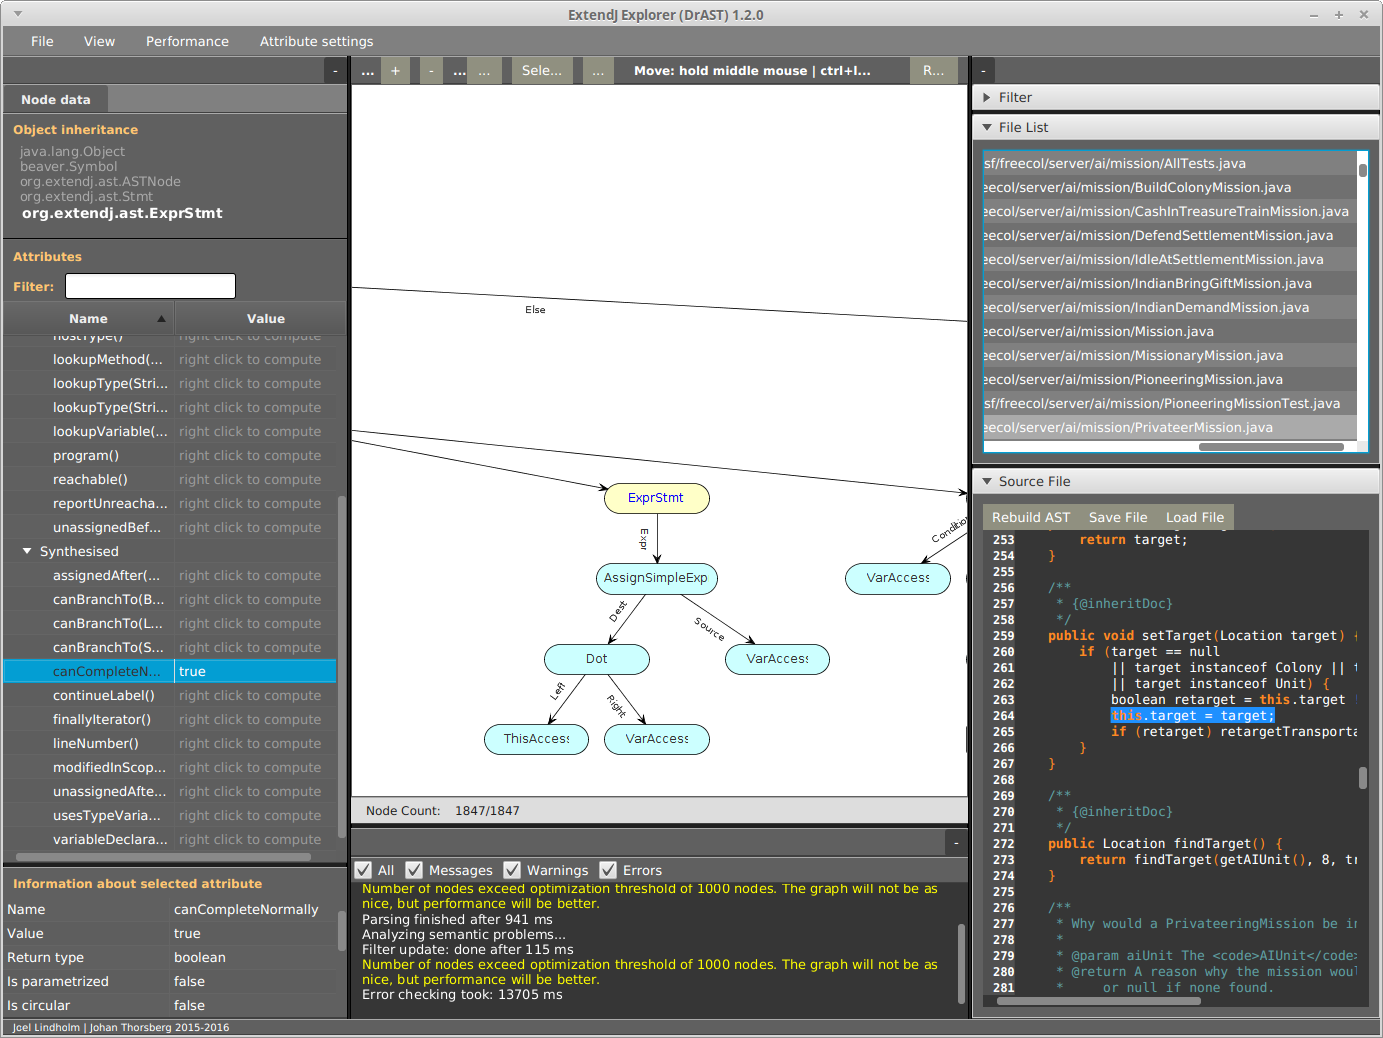
\includegraphics[width=1.0\textwidth]{figures/drast}
  \caption{
    Screenshot of DrAST extended with ExtendJ.
    The center part of the window contains a graph of the AST of one source file in
    freecol-0.10.7.
    The left part of the window contains a list of all attributes in the currently
    selected node. The \texttt{canCompleteNormally()} attribute has been selected and manually
    computed by the user.
    The right side of the window contains a list of all files in freecol-0.10.7,
    and below that is a source file view of the currently selected file.
    The bottom center part of the window shows status messages from DrAST. Note the
    message about compile-time error checking at the end.
    No compile-time errors or warnings were present in freecol-0.10.7.
  }
  \label{fig:screenshot1}
\end{figure}
\end{minipage}

}
